\clearpage
\bookpart{数学对象、计数与极限}{Objects, Counting and Limits}
\label{part:mathematical-language-analysis-optimization}

\BookPartGuide{%
本部分建立全书共同使用的基础对象、有限计数、集合大小的比较与极限语言，为线性空间、微积分与优化提供记号和推理起点。

第~\ref{chap:sets-relations-maps}章“集合、关系与映射”规定集合的描述与运算、二元关系及其分类与比较、映射及其单射满射双射，
并用索引族组织一批对象，以有限累计、数学归纳与递归处理有限多项的汇总与逐项生成；向量与矩阵留待线性空间部分与线性运算一起建立。
第~\ref{chap:counting}章“计数”以双射说明有限集合的元素个数，由分类、分步、对应、容斥与递推计算有限集合的大小。
第~\ref{chap:cardinality}章“基数”用双射和单射比较任意集合的大小，证明幂集总严格更大，
区分可数集与不可数集，为后文的可数覆盖与可数求和提供基础。
第~\ref{chap:function-limits}章“函数的极限”先建立实值函数的运算、函数族以及实数的确界与完备性，
再用数列极限精确说明“趋近”，建立级数的收敛与函数极限，并给出实轴上的邻域、开闭集与闭区间的紧致性，作为一元微积分的入口；
一般度量空间中的收敛条件在后续“空间与几何”部分的“度量空间”章给出。

本部分只建立对象、记号与极限语言，不展开线性运算、微分积分或求解算法；
后续部分在这些对象上分别建立空间结构、变化率、积分与极值。}

\chapter{集合、关系与映射}
\label{chap:sets-functions-and-proofs}
\label{chap:sets-relations-maps}

设想一所学校开设四门课程，几名学生各自选了其中几门。拿到这份选课记录，会问：
哪些课程有人选，哪些课程两人都选了；某名学生与某门课程之间有没有选课联系；
怎样把每名学生对应到自己的选课；记录编号以后怎样汇总各门课的人数。
要据此推理和计算，需要先说清讨论哪些对象、对象之间有什么联系、
怎样把一个对象对应到另一个对象，以及怎样给一批对象编号并累计。

本章依次建立这些工具。集合规定讨论范围，集合运算组合成员条件；
关系把成对的联系记录为有序对的集合，其中等价关系用来分类，偏序用来比较；
映射是每个输入恰有一个输出的关系，单射、满射与双射刻画两个集合的元素能否逐一配对；
索引族用映射给一批对象编号，有限累计、数学归纳与递归处理有限多项的汇总和逐项生成。
下一章用双射和有限累计计数，第~\ref{chap:cardinality}章再用映射比较无限集合的大小。

\section{集合的定义与运算}
\label{sec:prelim-sets-relations-functions}

本节先说明怎样写出集合、怎样判断两个集合相等，再定义集合运算，
最后用已有集合构造幂集与笛卡尔积。

\subsection{集合的定义和描述}
\label{sec:prelim-set-definition}

\paragraph{集合与元素}
由一些确定的对象组成的整体称为\term{集合}（set），其中的对象称为它的元素；
“确定”是说任给一个对象，都能判断它是不是其中的元素。例如四门课程的编号组成集合$\{1,2,3,4\}$。
若$x$是集合$X$的元素，就说$x$属于$X$，记作$x\in X$；否则记作$x\notin X$。
集合只由它含有哪些元素决定：含有相同元素的两个集合相等，记作$X=Y$。
因此$\{1,2,3\}$、$\{3,2,1\}$与$\{1,1,2,3\}$是同一个集合。
不含任何元素的集合称为空集，记作$\varnothing$；只含一个元素$a$的集合$\{a\}$称为单元素集。

\paragraph{集合的描述}
列举法把元素逐个写在花括号中，例如$U=\{1,2,3,4\}$；
描述法写出挑选范围和所满足的条件，例如$U=\{i\in\mathbb Z:1\leq i\leq4\}$，
冒号读作“使得”，冒号前的$i\in\mathbb Z$表示从整数中挑选。挑选范围不能省略：
同一条件下从实数中挑选，得到的是区间$\{x\in\mathbb R:1\leq x\leq4\}=[1,4]$。
本书用$\mathbb N=\{0,1,2,\ldots\}$表示自然数集合，$\mathbb N_+=\{1,2,\ldots\}$表示正整数集合，
$\mathbb Z$、$\mathbb Q$和$\mathbb R$分别表示整数、有理数与实数集合；
区间$[a,b]$包含两个端点，$(a,b)$不含端点，$[a,b)$与$(a,b]$各只含一个端点。

\paragraph{子集}
若$A$的每个元素都属于$B$，就称$A$是$B$的子集（subset），记作$A\subseteq B$；
若还有$A\neq B$，就称$A$是$B$的真子集，记作$A\subsetneq B$。
属于与包含比较的对象不同：$1\in U$说的是编号$1$属于$U$，$\{1\}\subseteq U$说的是集合$\{1\}$包含于$U$；
$\{1,2\}\subseteq U$成立，$\{1,2\}\in U$却不成立，因为$U$的元素是编号而不是集合。
空集是任何集合的子集，因为“它的每个元素都属于$B$”无从违反。
由于集合只由元素决定，$A=B$当且仅当$A\subseteq B$且$B\subseteq A$；
证明集合相等时，常把等式拆成这两个包含分别验证，称为双向包含。

\subsection{集合的运算}
\label{sec:prelim-set-operations}

\paragraph{基本运算}
设甲、乙两名学生的选课分别是$C=\{1,2,3\}$与$D=\{2,3,4\}$，以全部课程$U=\{1,2,3,4\}$为全集。
合并名单、找共同课程、排除已知课程，分别对应下面的运算。
\begin{itemize}
 \item 并集：$X\cup Y=\{x:x\in X\text{ 或 }x\in Y\}$，“或”允许两个条件同时成立。例如$C\cup D=\{1,2,3,4\}$。
 \item 交集：$X\cap Y=\{x:x\in X\text{ 且 }x\in Y\}$，例如$C\cap D=\{2,3\}$。若$X\cap Y=\varnothing$，称$X$与$Y$不交。
 \item 差集：$X\setminus Y=\{x:x\in X\text{ 且 }x\notin Y\}$，例如$C\setminus D=\{1\}$，而$D\setminus C=\{4\}$。
 \item 对称差：$X\mathbin{\triangle}Y=(X\setminus Y)\cup(Y\setminus X)$，即恰好属于其中一个集合的元素，例如$C\mathbin{\triangle}D=\{1,4\}$。
 \item 补集：对全集$U$的子集$X$，$X^{\mathrm c}=U\setminus X$，例如$C^{\mathrm c}=\{4\}$。
       补集依赖全集：若全集换成$\{1,2,3,4,5\}$，$C$的补集就变成$\{4,5\}$。
\end{itemize}

\paragraph{运算律}
这些运算都由成员条件定义，运算律可以逐个元素核对。交与并满足交换律、结合律与分配律：
\begin{align*}
 X\cap Y&=Y\cap X,\\
 X\cup Y&=Y\cup X,\\
 (X\cap Y)\cap Z&=X\cap(Y\cap Z),\\
 (X\cup Y)\cup Z&=X\cup(Y\cup Z),\\
 X\cap(Y\cup Z)&=(X\cap Y)\cup(X\cap Z),\\
 X\cup(Y\cap Z)&=(X\cup Y)\cap(X\cup Z).
\end{align*}
前四式来自“且”“或”可以交换次序、改变组合方式。以第五式为例，左边要求$x\in X$，并且$x$属于$Y$或$Z$；
这恰好是说$x$同时属于$X$与$Y$，或者同时属于$X$与$Z$。
补集与交、并的关系由下面的定理给出。
\begin{theorem}[De Morgan律]
\label{thm:sets-de-morgan}
设$X,Y$是全集$U$的子集，则
\begin{equation}
 (X\cup Y)^{\mathrm c}=X^{\mathrm c}\cap Y^{\mathrm c},\qquad
 (X\cap Y)^{\mathrm c}=X^{\mathrm c}\cup Y^{\mathrm c}.
 \label{eq:prelim-de-morgan-two-sets}
\end{equation}
\end{theorem}
\begin{proof}
用双向包含证明第一式。若$u\in(X\cup Y)^{\mathrm c}$，则$u\notin X\cup Y$，因而$u\notin X$且$u\notin Y$，
即$u\in X^{\mathrm c}\cap Y^{\mathrm c}$。反过来，若$u\in X^{\mathrm c}\cap Y^{\mathrm c}$，则$u$既不属于$X$也不属于$Y$，
因而$u\notin X\cup Y$，即$u\in(X\cup Y)^{\mathrm c}$。
第二式同理：$u\notin X\cap Y$当且仅当$u\notin X$或$u\notin Y$，即$u\in X^{\mathrm c}\cup Y^{\mathrm c}$。
\end{proof}
第一式说的是，“不满足任何一个条件”与“每个条件都不满足”是同一件事；下一章计数违反限制的结果时要用到它。

\paragraph{差集的次序}
差集既没有交换律，也没有结合律。前面已有$C\setminus D\neq D\setminus C$；再取$E=\{1\}$，
则$(C\setminus D)\setminus E=\varnothing$，而$C\setminus(D\setminus E)=C\setminus D=\{1\}$。
所以连续求差时必须用括号标明先后。

\subsection{幂集、笛卡尔积与有序组}
\label{sec:sets-power-sets-products}

前面的运算得到的仍是原全集的子集。把一名学生的全部选课当成一个对象，
或者把“先选一门、再选一门”记录成一个对象，则需要构造新的集合。

\paragraph{幂集}
集合$X$的全部子集组成的集合称为$X$的\term{幂集}（power set），记作
\[
 \mathcal P(X)=\{A:A\subseteq X\}.
\]
例如$\mathcal P(\{1,2\})=\{\varnothing,\{1\},\{2\},\{1,2\}\}$，一名学生的全部可能选课就是课程集合的幂集。
幂集的元素是集合：$\{1\}\in\mathcal P(\{1,2\})$，而$1$不是$\mathcal P(\{1,2\})$的元素。
以集合为元素的集合也称为\term{集合族}（set family），它不必收集全部子集，例如$\{\{1\},\{2\}\}\subseteq\mathcal P(\{1,2\})$。
有限集合的幂集有多少个元素，留到下一章计算。

\paragraph{有序对与笛卡尔积}
集合不记录次序，有序对$(x,y)$则保留两个位置：$(x,y)=(x',y')$要求$x=x'$且$y=y'$。
所以$(1,2)\neq(2,1)$，而$\{1,2\}=\{2,1\}$；有序对还允许两个位置相同，如$(1,1)$。
第一个位置取自$X$、第二个位置取自$Y$的全部有序对组成\term{笛卡尔积}（Cartesian product）
\[
 X\times Y=\{(x,y):x\in X,\ y\in Y\}.
\]
例如$\{1,2\}\times\{a,b\}=\{(1,a),(1,b),(2,a),(2,b)\}$。当$X,Y$都非空且$X\neq Y$时，$X\times Y\neq Y\times X$。

一般地，有序$d$元组$(x_1,\ldots,x_d)$的第$i$个位置称为第$i$个坐标，两个$d$元组相等当且仅当对应坐标逐一相等。
第$i$个坐标取自$X_i$的全部$d$元组组成$X_1\times\cdots\times X_d$，各因子相同时记为$X^d$；
特别地，$\mathbb R^d$是全部有序$d$元实数组的集合，$\mathbb R^2$就是平面上点的坐标。
映射$(x_1,\ldots,x_d)\mapsto x_i$称为第$i$个投影。下一节的关系就是笛卡尔积的子集。

\section{关系与分类}
\label{sec:prelim-binary-relations}

“学生选了某门课”“$1$不大于$2$”“两个整数除以$3$的余数相同”，问的都是一对对象是否满足某个条件。
本节把这样的条件写成有序对的集合，研究关系的性质，再用两类特殊的关系分类和比较。

\subsection{二元关系及其性质}
\label{sec:prelim-binary-relation-definition}
\label{sec:prelim-relation-properties}

\paragraph{二元关系}
设三名学生$s_1,s_2,s_3$中，$s_1$选了课程$1,2,3$，$s_2$选了$2,3,4$，$s_3$没有选课。
选课情况是笛卡尔积$\{s_1,s_2,s_3\}\times\{1,2,3,4\}$的子集
\[
 R=\{(s_1,1),(s_1,2),(s_1,3),(s_2,2),(s_2,3),(s_2,4)\}.
\]
一般地，笛卡尔积的任一子集$R\subseteq X\times Y$称为$X$到$Y$的\term{二元关系}（binary relation），
写$xRy$表示$(x,y)\in R$；$X=Y$时称$R$为$X$上的关系。
至少与一个$y$有关系的$x$组成$R$的定义域，至少与一个$x$有关系的$y$组成$R$的值域；
上例的定义域是$\{s_1,s_2\}$，值域是全部四门课程。同一对集合之间可以有许多关系，空集和整个积也是关系；
关系也不要求每个$x$恰好对应一个$y$：$s_1$对应三门课，$s_3$一门也不对应。

\paragraph{关系的基本性质}
设$R$是集合$X$上的关系。
若每个$x\in X$都有$xRx$，称$R$具有\term{自反性}（reflexivity）；
若$xRy$总蕴含$yRx$，称$R$具有\term{对称性}（symmetry）；
若$xRy$与$yRx$只在$x=y$时同时成立，称$R$具有\term{反对称性}（antisymmetry）；
若$xRy$且$yRz$总蕴含$xRz$，称$R$具有\term{传递性}（transitivity）。

用三个熟悉的关系核对：
\begin{itemize}
 \item 相等关系：四种性质都有，因为它只关联同一个对象。
 \item 实数上的$\leq$：自反、反对称、传递，但不对称，因为$1\leq2$而$2\not\leq1$。
 \item 正整数上的整除$a\mid b$（存在正整数$c$使$b=ac$）：自反（$a=a\cdot1$）；传递（由$b=ac$、$e=bc'$得$e=a(cc')$）；
       反对称（$a\mid b$且$b\mid a$时$a\leq b\leq a$）；不对称。若放到非零整数上，$2\mid-2$且$-2\mid2$，反对称性不再成立。
\end{itemize}
最后一例说明，同一条规则是否具有某种性质，还取决于在哪个集合上讨论。

反对称性不是对称性的否定。若$xRy$成立时$yRx$总不成立，称$R$具有\term{非对称性}（asymmetry），
例如实数上的$<$；$\leq$不是非对称的，因为$1\leq1$。非对称关系一定反对称，
并且没有$x$满足$xRx$，即具有\term{反自反性}（irreflexivity）；反对称关系则允许$xRx$。

\paragraph{关系的闭包}
一个关系缺少某种性质时，可以补入必要的有序对。包含$R$、具有指定性质、并且在包含意义下最小的关系，
称为相应的\term{关系闭包}（closure of a relation）；“最小”是说任何包含$R$并具有该性质的关系都包含它。
反对称性不能靠补入有序对获得，因为已有的双向关联无法去掉。

自反闭包是$R\cup\{(x,x):x\in X\}$，对称闭包是$R\cup\{(y,x):(x,y)\in R\}$，补入的都是满足性质所必需的有序对。
例如$\{1,2,3\}$上的$\{(1,2),(2,3)\}$，自反闭包补入$(1,1),(2,2),(3,3)$，对称闭包补入$(2,1),(3,2)$。

传递闭包$R^+$规定：$xR^+y$当且仅当存在有限链$x=x_0,x_1,\ldots,x_n=y$（$n\geq1$），每一步都有$x_{k-1}Rx_k$。
两条链首尾相接仍是链，所以$R^+$传递；任何包含$R$的传递关系沿链使用传递性，都含有链的首尾对，所以$R^+$最小。
上例的传递闭包只需补入$(1,3)$。

\subsection{等价关系、划分与商集}
\label{sec:prelim-equivalence-relations}

\paragraph{等价关系}
按除以$3$的余数可以把整数分成三组。“分在同一组”这一关系应当满足：每个整数与自己同组；
$x$与$y$同组时$y$与$x$也同组；$x$与$y$、$y$与$z$分别同组时$x$与$z$也同组。这正是自反、对称与传递性。
\begin{definition}[等价关系]
\label{def:prelim-equivalence-relation}
设$R$是集合$X$上的关系。若$R$具有自反性、对称性与传递性，就称$R$为\term{等价关系}（equivalence relation）。
对$x\in X$，与$x$等价的元素组成$x$的\term{等价类}（equivalence class）
$[x]_R=\{y\in X:yRx\}$，$x$称为这个等价类的一个代表元。
\end{definition}
整数上的关系“$3$整除$x-y$”是等价关系：$x-x=0$；$x-y$是$3$的倍数时$y-x$也是；
$x-y$与$y-z$都是$3$的倍数时，它们的和$x-z$也是。它有三个等价类$[0],[1],[2]$，而$[3]=[0]$，
同一个等价类可以由不同的代表元写出。

\paragraph{等价类与划分}
若$X$的一族非空子集两两不交，并且它们的并等于$X$，就称这族子集为$X$的一个\term{划分}（partition）。
等价关系恰好给出划分。
\begin{theorem}[等价类构成划分]
\label{thm:sets-equivalence-partition}
设$R$是集合$X$上的等价关系，则全部等价类组成$X$的一个划分；并且对$x,y\in X$，或者$[x]_R=[y]_R$，或者$[x]_R\cap[y]_R=\varnothing$。
反过来，$X$的每个划分都由唯一的等价关系这样给出，即“属于同一块”。
\end{theorem}
\begin{proof}
由自反性，$x\in[x]_R$，所以每个等价类非空，并且各等价类的并是$X$。
设$z\in[x]_R\cap[y]_R$，即$zRx$且$zRy$。由对称性得$xRz$，再由传递性得$xRy$。
于是任取$u\in[x]_R$，由$uRx$与$xRy$得$uRy$，即$u\in[y]_R$，所以$[x]_R\subseteq[y]_R$；交换$x,y$得反向包含。
因此有公共元素的两个等价类相等，不同的等价类两两不交，全部等价类构成划分。
反过来，给定划分，令$xRy$当且仅当$x,y$属于同一块，三条性质直接成立，其等价类就是各块；
而任何以这些块为等价类的等价关系都必须如此定义，所以它唯一。
\end{proof}
因此，在同一个集合上给出等价关系与给出划分是同一件事的两种写法。

\paragraph{商集}
分组以后，常把每一组当作一个新对象。全部等价类组成的集合记为$X/R$，称为商集（quotient set）。
对整数按除以$3$的余数分组，商集是$\{[0],[1],[2]\}$；它的三个元素都是整数的子集，不是整数，
$0,1,2$只是用来写出它们的代表元。

正因为代表元只是记法，在商集上定义运算或映射时，必须检查结果不依赖代表元的选取。
例如规定$[a]+[b]=[a+b]$：若$a'\in[a]$、$b'\in[b]$，则$(a'+b')-(a+b)$仍是$3$的倍数，结果不变，所以这一加法有意义。
规定“$[a]$的奇偶性就是$a$的奇偶性”则不行：$0$与$3$代表同一个等价类，奇偶性却不同。

商集的元素也可以有几何含义。在平面上除原点以外的点中，规定$P\sim Q$当且仅当存在非零实数$c$使$P=cQ$，
这是等价关系，每个等价类是一条过原点的直线去掉原点；若只允许$c>0$，同一直线在原点两侧的部分分属两个类。
图~\ref{fig:vol1-add-equivalence-directions}比较这两种分类。
\begin{figure}[!htb]
  \centering
  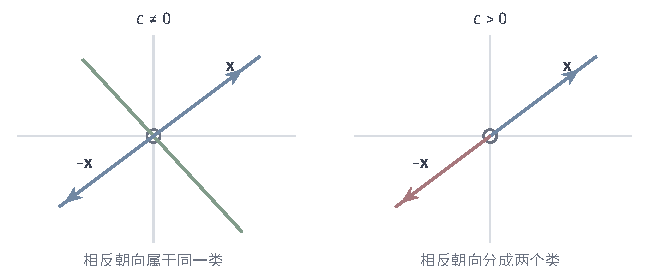
\includegraphics[width=112mm]{figures/01-mathematical-preliminaries-upper/00-shared/tikz/mathematical-language-combinatorics-analysis-optimization-comprehension-additions/equivalence-directions.pdf}
  \caption{平面中非原点的等价分类。每支箭头从原点指向一个点。左侧允许非零实比例，同一直线上的点属于同一类；右侧只允许正比例，同一直线的两侧分成蓝、红两类。绿色表示另一条直线上的类；空心原点不属于被分类的集合。}
  \label{fig:vol1-add-equivalence-directions}
\end{figure}

\subsection{偏序、全序与极值元素}
\label{sec:prelim-order-relations}

\paragraph{偏序与全序}
子集之间可以按包含比较，正整数之间可以按整除比较，但$\{1\}$与$\{2\}$互不包含，$2$与$3$互不整除。
这类比较关系都具有自反性、反对称性与传递性。
\begin{definition}[偏序关系]
\label{def:prelim-partial-order}
集合$X$上具有自反性、反对称性与传递性的关系称为\term{偏序关系}（partial order），常记作$\preceq$，
配备了偏序的集合记作$(X,\preceq)$。若$x\preceq y$与$y\preceq x$至少有一个成立，称$x$与$y$可比较。
若$X$中任意两个元素都可比较，则称$\preceq$为\term{全序}（total order）。
\end{definition}
实数上的$\leq$是全序，包含关系与整除关系只是偏序。

\paragraph{最小元与极小元}
设$A\subseteq X$非空。若$a\in A$满足$a\preceq b$对每个$b\in A$成立，称$a$为$A$的\term{最小元}（least element）；
若$b\preceq a$对每个$b\in A$成立，称$a$为\term{最大元}（greatest element）。
若$b\in A$且$b\preceq a$必有$b=a$，即$A$中没有比$a$更小的元素，称$a$为\term{极小元}（minimal element）；
若$b\in A$且$a\preceq b$必有$b=a$，称$a$为\term{极大元}（maximal element）。

在整除偏序下取$A=\{2,3,4,6\}$：$2,3$都是极小元，$4,6$都是极大元，但$A$没有最小元和最大元，因为$2$与$3$不可比，$4$与$6$也不可比。
最小元若存在则唯一：两个最小元彼此不大于对方，由反对称性相等。最小元一定是极小元；在全序中，极小元也是最小元。

\paragraph{上界与下界}
若$u\in X$满足$a\preceq u$对每个$a\in A$成立，称$u$为$A$的\term{上界}（upper bound）；
若$l\in X$满足$l\preceq a$对每个$a\in A$成立，称$l$为$A$的\term{下界}（lower bound）。
与最值元素不同，界不必属于$A$：上例中$12$是$A$的上界，$1$是下界，都不在$A$中。
全部上界中是否有最小的一个，一般偏序并不保证；实数集合的这一问题引出确界与完备性，见第~\ref{sec:prelim-optimal-values-errors}节。

\section{映射}
\label{sec:prelim-functions-value-ranges}

关系允许一个对象对应多个对象，也允许不对应任何对象。“每名学生的学号”“每个实数的平方”则要求每个输入恰好得到一个输出。
本节定义这种映射，研究像与原像，按能否逐一配对给映射分类，最后讨论复合与逆映射。

\subsection{映射、像与原像}
\label{sec:prelim-function-definition}

\paragraph{映射的定义}
设$X,Y$是两个集合。若$X$到$Y$的关系使每个$x\in X$恰好与一个$y\in Y$有关系，
就称它为$X$到$Y$的\term{映射}（map），也称\term{函数}（function），记作$f:X\to Y$；
与$x$对应的元素记作$f(x)$，记号$x\mapsto f(x)$读作“把$x$对应到$f(x)$”。
$X$称为定义域或源集，$Y$称为陪域或目标集，集合$\{(x,f(x)):x\in X\}$称为$f$的图像（graph）。
实际取得的输出组成$f(X)=\{f(x):x\in X\}$，称为值域或像集，它是目标集的子集。

上一节的选课关系不是映射：$s_1$对应三门课，$s_3$不对应任何课。实数上的$x\mapsto x^2$则是映射。

给出映射要同时说明源集、目标集和对应规则。同一规则$x\mapsto x^2$可以给出$\mathbb R\to\mathbb R$与$\mathbb R\to[0,\infty)$两个映射，
值域都是$[0,\infty)$，但前者的目标集中还有取不到的负数。两个映射相等，要求源集、目标集分别相同，且在每个输入处取值相同。
从$X$到$Y$的全部映射组成的集合记为$Y^X$，例如$\{0,1\}^{\{1,2\}}$有四个元素，由$(f(1),f(2))$的四种取值确定。

\paragraph{像与原像}
对映射$f:X\to Y$，可以问一组输入得到哪些输出，也可以问一组输出来自哪些输入。
对$A\subseteq X$与$B\subseteq Y$，分别定义$A$的像与$B$的\term{原像}（preimage）：
\begin{equation}
 f(A)=\{f(x):x\in A\}\subseteq Y,\qquad
 f^{-1}(B)=\{x\in X:f(x)\in B\}\subseteq X.
 \label{eq:prelim-preimage}
\end{equation}
对平方映射$f:\mathbb R\to\mathbb R$，$f(\{-2,1\})=\{1,4\}$，$f^{-1}(\{1\})=\{-1,1\}$，$f^{-1}([1,4])=[-2,-1]\cup[1,2]$，$f^{-1}(\{-1\})=\varnothing$。
原像是集合，可以含多个元素，也可以为空；记号$f^{-1}(B)$并不要求$f$有逆映射。
原像与集合运算相容：对$B,B'\subseteq Y$，
\begin{align*}
 f^{-1}(B\cup B')&=f^{-1}(B)\cup f^{-1}(B'),\\
 f^{-1}(B\cap B')&=f^{-1}(B)\cap f^{-1}(B'),\\
 f^{-1}(Y\setminus B)&=X\setminus f^{-1}(B).
\end{align*}
像只保持并，对交集一般只有$f(A\cap A')\subseteq f(A)\cap f(A')$。平方映射把$-1$与$1$都送到$1$，
于是$f(\{-1\}\cap\{1\})=\varnothing$，而$f(\{-1\})\cap f(\{1\})=\{1\}$。

\subsection{单射、满射与双射}
\label{sec:prelim-function-types}

对映射$f:X\to Y$，若不同输入的输出总不相同，即$f(x_1)=f(x_2)$必推出$x_1=x_2$，称$f$为\term{单射}（injection）；
若每个$y\in Y$都至少是一个输入的输出，即$f(X)=Y$，称$f$为\term{满射}（surjection）；
既单又满的映射称为\term{双射}（bijection）。

这些性质依赖源集和目标集。平方映射$\mathbb R\to\mathbb R$既不是单射也不是满射；
把目标集缩小为$[0,\infty)$，它成为满射；再把源集限制为$[0,\infty)$，它成为双射。
双射把两个集合的元素一一配对，说明它们“一样多”；单射把$X$的元素放进$Y$的不同位置，说明$X$“至多与$Y$一样多”。
下一章用双射计数，第~\ref{chap:cardinality}章用这两种比较研究无限集合。

\subsection{复合映射与逆映射}
\label{sec:prelim-map-operations}

\paragraph{复合与恒等映射}
对$f:X\to Y$与$g:Y\to Z$，定义\term{复合}（composition）映射$g\circ f:X\to Z$为
\[
 (g\circ f)(x)=g(f(x)).
\]
复合要求$f$的输出都在$g$的源集中；例如$g(u)=\sqrt u$定义在$[0,\infty)$上，$f(x)=x-1$只有限制在$x\geq1$上才能与它复合。

复合一般不能交换次序：$f(x)=x^2$、$g(x)=x+1$时，$(g\circ f)(1)=2$，而$(f\circ g)(1)=4$。

但复合满足结合律：对$h:Z\to W$，逐层代入得$(h\circ(g\circ f))(x)=h(g(f(x)))=((h\circ g)\circ f)(x)$，所以
\[
 h\circ(g\circ f)=(h\circ g)\circ f.
\]
单射的复合是单射，满射的复合是满射，因而双射的复合是双射。

映射$\operatorname{id}_X:X\to X$，$\operatorname{id}_X(x)=x$，称为恒等映射；对$f:X\to Y$有$f\circ\operatorname{id}_X=f=\operatorname{id}_Y\circ f$。
若先做一步、再做另一步的复合是恒等映射，第二步就撤销了第一步。

\paragraph{逆映射}
\phantomsection
\label{def:prelim-invertible-map}
撤销$f:X\to Y$，就是对每个$y\in Y$找回唯一的输入。若$f$是双射，满射保证这样的输入存在，单射保证它唯一；
把$y$对应到这个输入，得到$f$的逆映射（inverse map）$f^{-1}:Y\to X$，它满足
\[
 f^{-1}\circ f=\operatorname{id}_X,\qquad f\circ f^{-1}=\operatorname{id}_Y.
\]
反过来，若存在$h:Y\to X$使$h\circ f=\operatorname{id}_X$且$f\circ h=\operatorname{id}_Y$，则$f$是双射：
由$f(x_1)=f(x_2)$两边作用$h$得$x_1=x_2$；每个$y$都等于$f(h(y))$。
所以双射恰好是具有双侧逆映射的映射。例如$[0,\infty)\to[0,\infty)$的$x\mapsto x^2$的逆映射是$y\mapsto\sqrt y$。

逆映射与原像不同：原像对任何映射都有定义，作用在集合上；逆映射只对双射存在，作用在元素上。
对双射，$f^{-1}(\{y\})=\{f^{-1}(y)\}$，两者一致。图~\ref{fig:prelim-preimage-inverse}比较这两种反向操作。
若$f:X\to Y$与$g:Y\to Z$都是双射，则
\begin{equation}
 (g\circ f)^{-1}=f^{-1}\circ g^{-1},
 \label{eq:prelim-inverse-composition}
\end{equation}
因为由结合律$(f^{-1}\circ g^{-1})\circ(g\circ f)=f^{-1}\circ f=\operatorname{id}_X$，另一侧同理。
例如先平方、再加$1$把$x\geq0$送到$z=x^2+1$，撤销时先减$1$、再开平方。
后两章将反复用双射的复合换掉难数的集合、证明两个集合等势。

\begin{figure}[htbp]
  \centering
  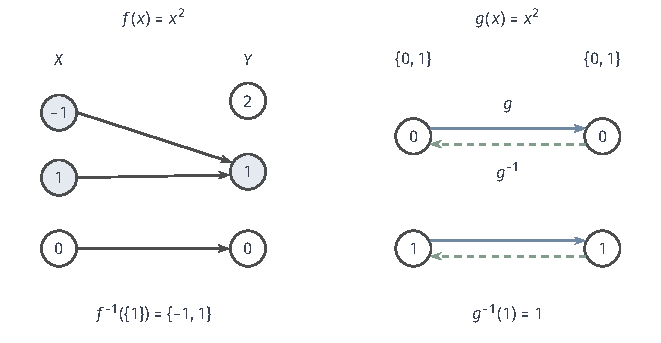
\includegraphics[width=112.0mm]{figures/01-mathematical-preliminaries-upper/01-mathematical-language-combinatorics-analysis-optimization/tikz/prelim-preimage-inverse/figure.pdf}
  \caption{原像与逆映射回答不同问题。左侧$f:\{-1,0,1\}\to\{0,1,2\}$按平方取值，
  标出的$1$有两个原输入，$2$没有原输入；原像$f^{-1}(\{1\})=\{-1,1\}$仍有定义。
  右侧将定义域与陪域都限制为$\{0,1\}$得到双射$g$，实线表示正向求值，虚线表示
  逆映射，因而$g^{-1}(1)=1$是一个元素。两侧均为精确的有限映射。}
  \label{fig:prelim-preimage-inverse}
\end{figure}

\section{索引族}
\label{sec:prelim-indices-sums-recurrences}

三次测验的得分是$1,1,4$，组成集合时只剩$\{1,4\}$，求总分时却要把两个$1$分别计入。
本节用映射给每次出现一个编号，再讨论一族集合的并与交、有限多个数的累计，以及归纳与递归。

\subsection{索引族的定义}
\label{sec:prelim-indexed-sequences}

\paragraph{索引族}
给每次测验一个编号，再为每个编号指定得分，就是一个映射。
\begin{definition}[索引族]
\label{def:prelim-indexed-family}
给定索引集合$I$和对象集合$X$，映射$a:I\to X$也称为以$I$为索引的\term{索引族}（indexed family），
把$a(i)$记作$a_i$，整个族记作$(a_i)_{i\in I}$。$i$称为指标，$a_i$称为指标$i$对应的对象。
\end{definition}
测验得分写成$a_1=1$、$a_2=1$、$a_3=4$。不同指标可以对应相同的对象，所以索引族与取值集合$\{a_i:i\in I\}=\{1,4\}$不同：
前者保留每一次出现，后者只记录出现过哪些值。

\paragraph{序列}
按正整数顺序索引的族称为序列（sequence）：只取$1,\ldots,n$时是有限序列，取全部正整数时是无限序列；
取值为实数的序列称为数列，例如$(1/n)_{n\geq1}$。从$0$开始编号时写$(a_n)_{n\geq0}$。
记录逐步更新的结果时，把第$t$步的结果记作$a^{(t)}$，用带括号的上标表示步数，以区别于幂$a^t$。

\paragraph{二维索引族与集合族}
两个指标共同指定一个对象时，得到二维索引族$(a_{i,j})_{(i,j)\in I\times J}$。
例如$a_{i,j}=3(i-1)+j$（$i=1,2$，$j=1,2,3$）排成两行$(1,2,3)$与$(4,5,6)$，固定$i$得到一行，固定$j$得到一列。
对象也可以是集合，例如三名学生的选课$(S_i)_{i\in\{1,2,3\}}$。这样的族记录的是每份选课，
不能与全部选课的并混为一谈：$S_1=\{1,2\}$、$S_2=\{2\}$时，并集$\{1,2\}$只记录哪些课程有人选过。

\subsection{集合族的运算}
\label{sec:prelim-indexed-set-operations}

给定全集$U$的子集族$(A_i)_{i\in I}$，“至少属于一个成员”和“属于每个成员”分别定义索引并与索引交：
\[
 \begin{aligned}
  \bigcup_{i\in I}A_i&=\{u\in U:\text{存在 }i\in I\text{ 使 }u\in A_i\},\\
  \bigcap_{i\in I}A_i&=\{u\in U:\text{对每个 }i\in I\text{ 都有 }u\in A_i\}.
 \end{aligned}
\]
$I=\{1,2\}$时回到$A_1\cup A_2$与$A_1\cap A_2$；$I=\mathbb N_+$时也写成$\bigcup_{n=1}^\infty A_n$与$\bigcap_{n=1}^\infty A_n$。
按定义，空族的交是全集$U$，空族的并是空集。De Morgan律对任意索引族同样成立：
\begin{equation}
 \Bigl(\bigcup_{i\in I}A_i\Bigr)^{\mathrm c}=\bigcap_{i\in I}A_i^{\mathrm c},\qquad
 \Bigl(\bigcap_{i\in I}A_i\Bigr)^{\mathrm c}=\bigcup_{i\in I}A_i^{\mathrm c},
 \label{eq:prelim-de-morgan-families}
\end{equation}
证明与定理~\ref{thm:sets-de-morgan}相同：不存在$i$使$u\in A_i$，就是对每个$i$都有$u\in A_i^{\mathrm c}$。

在$U=[0,1]$中取递增族$A_n=[1/n,1]$，则$\bigcup_{n\geq1}A_n=(0,1]$：每个$x>0$在$n\geq1/x$时属于$A_n$，而$0$不属于任何$A_n$。
取递减族$B_n=[0,1/n)$，则$\bigcap_{n\geq1}B_n=\{0\}$。成员都是区间，无限并却缺了端点，无限交只剩一个点；后面测量集合时还会遇到这类现象。

\subsection{有限累计}
\label{sec:prelim-finite-sums-products}

\paragraph{有限和与有限积}
对$n\geq1$个数$a_1,\ldots,a_n$，记
\[
 \sum_{i=1}^{n}a_i=a_1+\cdots+a_n,\qquad \prod_{i=1}^{n}a_i=a_1\cdots a_n.
\]
这两个记号只是有限次运算的缩写，可以逐项规定：$\sum_{i=1}^{n+1}a_i=\sum_{i=1}^na_i+a_{n+1}$，积同理。
逐项规定需要起点，约定空和为$0$、空积为$1$：
\[
 \sum_{i\in\varnothing}a_i=0,\qquad \prod_{i\in\varnothing}a_i=1,
\]
这样把一组项拆成两部分分别汇总时，即使一部分为空，结果也不变。
对有限索引集合$I$，也写$\sum_{i\in I}a_i$与$\prod_{i\in I}a_i$；这些记号在整数、有理数、实数中含义相同。

\paragraph{索引与有限换序}
求和变量的名称不影响结果：$\sum_{i=1}^na_i=\sum_{k=1}^na_k$，这里的$i$称为\term{哑索引}（dummy index）。
自由索引则留在结果中：在$b_j=\sum_{i=1}^{n}x_{i,j}$中，$j$须固定才知道汇总的是哪一列，
所以可以把$i$改为$k$，却不能只改右边的$j$，也不能把$i$改名为已占用的$j$。
平移哑索引时，范围要随之改写：$\sum_{n=1}^{N}b_{n+1}=\sum_{m=2}^{N+1}b_m$。

由加法、乘法的交换律、结合律与分配律，有限和满足线性关系
\[
 \sum_{i=1}^{n}(\alpha u_i+\beta v_i)=\alpha\sum_{i=1}^{n}u_i+\beta\sum_{i=1}^{n}v_i,
\]
有限积满足$\prod_{i=1}^n(a_ib_i)=\bigl(\prod_{i=1}^na_i\bigr)\bigl(\prod_{i=1}^nb_i\bigr)$与$\prod_{i=1}^n(ca_i)=c^n\prod_{i=1}^na_i$；
积没有线性关系，例如$(1+2)(3+4)\neq1\cdot3+2\cdot4$。结合平移与线性关系得到裂项求和：
\begin{equation}
 \sum_{n=1}^N(b_{n+1}-b_n)=\sum_{m=2}^{N+1}b_m-\sum_{n=1}^{N}b_n=b_{N+1}-b_1.
 \label{eq:prelim-telescoping-sum}
\end{equation}
例如由$\frac1{n(n+1)}=\frac1n-\frac1{n+1}$得$\sum_{n=1}^N\frac1{n(n+1)}=1-\frac1{N+1}$。

对二维有限数组$(a_{i,j})$，$i=1,\ldots,n$，$j=1,\ldots,d$，按行汇总与按列汇总相等：
\[
 \sum_{i=1}^{n}\sum_{j=1}^{d}a_{i,j}=\sum_{j=1}^{d}\sum_{i=1}^{n}a_{i,j},
\]
因为两边都把每个索引对恰好计入一次。内层范围依赖外层索引时，换序要重写范围，使遍历的仍是同一批索引对：
\begin{equation}
 \sum_{i=1}^{n}\sum_{j=1}^{i}a_{i,j}=\sum_{j=1}^{n}\sum_{i=j}^{n}a_{i,j},
 \label{eq:prelim-triangular-sum}
\end{equation}
两边都恰好遍历满足$1\leq j\leq i\leq n$的$(i,j)$；若把右边内层误写成$i=1,\ldots,n$，就会多算$j>i$的项。
这些换序依赖项数有限；无限多项的和要先用极限定义，不能由有限情形直接推广。

\subsection{数学归纳与递归}
\label{sec:prelim-recurrence-unrolling}

\paragraph{数学归纳}
设$\rho\neq1$，记$G_N=\sum_{n=0}^N\rho^n$（约定$\rho^0=1$）。由$G_0=1$、$G_1=\frac{1-\rho^2}{1-\rho}$、$G_2=\frac{1-\rho^3}{1-\rho}$，可以猜测
\begin{equation}
 \sum_{n=0}^N\rho^n=\frac{1-\rho^{N+1}}{1-\rho}\qquad(\rho\neq1),
 \qquad\sum_{n=0}^N1^n=N+1.
 \label{eq:prelim-finite-geometric-sum}
\end{equation}
验证前几项不能保证公式对每个$N$成立。\term{数学归纳法}（mathematical induction）给出证明方法：
要证明关于$N=0,1,2,\ldots$的命题$P(N)$全部成立，只需证明$P(0)$成立（归纳基础），
以及对每个$N\geq0$，由$P(N)$能推出$P(N+1)$（归纳步）；归纳步中假定成立的$P(N)$称为归纳假设。
对上式，$N=0$时两边都是$1$；若$G_N=\frac{1-\rho^{N+1}}{1-\rho}$，则
\[
 G_{N+1}=G_N+\rho^{N+1}=\frac{1-\rho^{N+1}+\rho^{N+1}-\rho^{N+2}}{1-\rho}=\frac{1-\rho^{N+2}}{1-\rho}.
\]
所以公式对每个$N$成立；$\rho=1$时每项都是$1$，和为$N+1$。

有时证明$P(N+1)$要用到此前的全部命题。强归纳法规定：若$P(0)$成立，并且对每个$N\geq0$，
由$P(0),\ldots,P(N)$全部成立能推出$P(N+1)$，则$P(N)$对一切$N$成立；把命题换成“$P(0),\ldots,P(N)$都成立”，它就回到普通归纳。
例如每个大于$1$的整数$m$都是素数之积：$m$是素数时成立；否则$m=ab$，$1<a,b<m$，由较早阶段的结论，$a,b$都是素数之积，于是$m$也是。

\paragraph{递归}
给定集合$X$、初值$x_0\in X$与更新映射$T:X\to X$，规定
\[
 x_{t+1}=T(x_t),\qquad t=0,1,2,\ldots,
\]
这种用已有的项确定下一项的定义方式称为\term{递推}（recurrence），也称递归定义；有限和的逐项规定就是一例。
递推确实确定了唯一的序列：称满足$y_0=x_0$且$y_{k+1}=T(y_k)$（$k<n$）的$(y_0,\ldots,y_n)$为长度$n+1$的初段，
对$n$归纳可知每个长度的初段恰有一个，且较短的初段是较长初段的开头部分；
令$x_n$为长度$n+1$的初段的末项即得所求序列，而任何满足递推的序列的前$n+1$项都是初段，因而与之相同。

递推定义对象，归纳证明它的性质。例如等比递推
\begin{equation}
 e^{(t+1)}=\rho e^{(t)},\qquad e^{(0)}=e_0,\qquad t=0,1,\ldots
 \label{eq:prelim-geometric-recurrence}
\end{equation}
在$e_0=8$、$\rho=1/2$时给出$8,4,2,1,\ldots$，提示通项$e^{(t)}=\rho^te_0$；
归纳验证：$t=0$时成立，若$e^{(t)}=\rho^te_0$，则$e^{(t+1)}=\rho^{t+1}e_0$。等差递推$a^{(t+1)}=a^{(t)}+d$同理得$a^{(t)}=a_0+td$。
由$|e^{(t+1)}|=|\rho|\,|e^{(t)}|$，$|\rho|<1$时非零项的绝对值逐步缩小，$|\rho|>1$时逐步放大，$\rho=-1$时大小不变、符号交替。
$t$无限增大时这些数怎样变化，要到第~\ref{chap:function-limits}章用极限回答。

\section{本章小结}
\label{sec:prelim-sets-functions-summary}

集合由元素决定，集合相等可以用双向包含证明，运算律与De Morgan律都能逐个元素核对，差集则没有交换律和结合律；
幂集收集全部子集，笛卡尔积记录有次序的多次选择。关系是笛卡尔积的子集：等价关系与划分是同一结构的两种写法，
商集上的运算必须与代表元无关；偏序允许对象互不可比，最小元与极小元、界与最值要分别判断。

映射要求每个输入恰有一个输出。原像保持并、交与补，像一般不保持交；单射、满射与双射依赖源集和目标集，
双射恰好具有双侧逆映射，逆映射作用于元素，原像作用于集合。索引族保留每次出现的编号，
有限和与有限积换序时须遍历同一批项；递推定义序列，归纳证明它的性质。

全章要分清对象本身与它的编号（索引）、等价类与代表元、映射与表示它的规则表达式。
下一章用双射把有限集合与$\{1,\ldots,n\}$配对，借助分类、分步、对应和递推计数；
第~\ref{chap:cardinality}章再用单射和双射比较无限集合的大小。实值函数的运算、确界和极限从第~\ref{chap:function-limits}章开始讨论。

\chapter{计数}
\label{chap:combinatorics}
\label{chap:counting}

从四门课中任选一些，共有多少种选法？从四名学生中选出组长和记录员，又有多少种安排？
对象稍多时，逐一列举既费力又容易重复或遗漏。本章研究怎样不逐一列举而算出有限集合的元素个数。

计数前先要确定什么算一个结果。从四个对象中依次取两个，$(1,3)$与$(3,1)$是不同的有序记录；
若只记录选中了哪些对象，它们都是子集$\{1,3\}$。记录方式不同，结果数也不同。
元素个数借助第~\ref{chap:sets-relations-maps}章的双射来说明：有限集合$A$有$n$个元素，是说存在双射$\{1,\ldots,n\}\to A$，
即能把$A$的元素恰好编号为$1,\ldots,n$；空集对应$n=0$。$A$的元素个数记为$|A|$。

本章先推出加法规则和乘法规则，再算出排列、组合、子集与划分的数量，最后用容斥原理处理类别重叠，用递推处理可化为更小同类问题的情形。
以下记$V=\{1,\ldots,n\}$，其中$n\geq0$。

\section{分类和分步计数}
\label{sec:comb-families-counting}
\label{sec:comb-finite-counting}
\label{sec:comb-decomposition-counting}
\label{sec:comb-classification-products}
\label{sec:comb-classification-counting}

本节的三条规则对应三种做法：把要数的集合换成更容易数的集合，把结果分成互不重叠的几类，把每个结果拆成依次进行的几步选择。

\paragraph{双射与计数}
数出有限集合$A$有$n$个元素，就是给出编号双射$g:\{1,\ldots,n\}\to A$。若另有双射$f:A\to B$，
则$f\circ g$把$B$的元素也恰好编号为$1,\ldots,n$。所以两个有限集合之间存在双射时，元素个数相同；
难数的集合可以换成与它一一对应的好数的集合。

同一个集合也不会数出两个不同的个数：若$h:\{1,\ldots,m\}\to\{1,\ldots,n\}$是双射，则$m=n$。
对$n$归纳：$n=0$时源集也只能为空，即$m=0$；$n\geq1$时$m\geq1$，设$h(j)=n$，交换$h$在$j$与$m$处的取值，
使$m$对应$n$，再把它限制到$\{1,\ldots,m-1\}$，得到到$\{1,\ldots,n-1\}$的双射，由归纳假设$m-1=n-1$。

\paragraph{加法规则}
若有限集合$A_1,\ldots,A_r$两两不交，则
\[
 \Bigl|\bigcup_{i=1}^r A_i\Bigr|=\sum_{i=1}^r|A_i|,
\]
这称为计数的加法规则。它来自编号的拼接：先给$A_1$的元素编号$1,\ldots,|A_1|$，再接着给$A_2$编号，依此类推；
两两不交保证没有元素被编号两次。使用时要检查各类覆盖全部结果且两两不交；类别重叠的情形留给第~\ref{sec:comb-overlap-counting}节的容斥原理。
由加法规则，若$B\subsetneq A$都是有限集合，则$|A|=|B|+|A\setminus B|>|B|$，即有限集合的真子集元素更少。

加法规则的一个推论是\term{抽屉原理}（pigeonhole principle）：把$m$个对象放进$k$个位置，若每个位置至多一个对象，
按位置分类得$m\leq k$；因此$m>k$时必有某个位置容纳至少两个对象。例如任选$13$人，必有两人同月出生。
换句话说，$m>k$时从$m$元集到$k$元集的映射都不是单射。

\paragraph{乘法规则}
\phantomsection
\label{sec:comb-stepwise-counting}
对有限集合$A_1,\ldots,A_r$，
\[
 |A_1\times\cdots\times A_r|=\prod_{i=1}^r|A_i|,
\]
这称为计数的乘法规则。$r=2$时，按第一个位置的取值把$A_1\times A_2$分成$|A_1|$类，
第$a$类$\{a\}\times A_2$与$A_2$之间有双射$(a,b)\mapsto b$，由加法规则得$|A_1|\cdot|A_2|$；一般的$r$对位置个数归纳。
例如第一位取$a,b$之一、第二位取$1,2,3$之一，共有$2\times3=6$个结果，逐一列出即$(a,1),(a,2),(a,3),(b,1),(b,2),(b,3)$；
长度为$n$的零一记录组成$\{0,1\}^n$，共$2^n$条。

分步选择中，后一步的选项常依赖前一步，例如先选组长、再从其余人中选记录员。
只要第$i$步在每种已有记录之后都恰有$n_i$个选项，完整记录数仍是$\prod_in_i$：按第一步分成$n_1$类，
每类由归纳假设都有$\prod_{i\geq2}n_i$个记录，再用加法规则。要求的是选项的个数固定，选项的内容可以变化。
若个数也随前一步改变，就先分类再相加。例如从四门课中选一门主修，主修课程$1$时只能从课程$2,3$中选辅修，
否则可从其余三门中选，完整记录数是$1\times2+3\times3=11$。

\section{排列与组合}
\label{sec:comb-permutation-combination-counts}
\label{sec:comb-subset-partition-counts}

选取若干对象时，可以记录它们所在的位置，也可以只记录选中了谁。先按位置计数，再把只是位置不同的记录归为一类，
就能联系这两类问题；不限选取个数或二分对象时，则可以借助零一记录。

\paragraph{排列数}
设$0\leq k\leq n$。从$n$个不同对象中取出$k$个依次放在$k$个位置上且不重复，所得有序$k$元组称为排列，个数记为$P(n,k)$。
各位置依次有$n,n-1,\ldots,n-k+1$种选择，由乘法规则
\[
 P(n,k)=\prod_{i=0}^{k-1}(n-i)=n(n-1)\cdots(n-k+1),
\]
$k=0$时为空积$1$，对应唯一的空排列。例如从四人中选组长和记录员有$P(4,2)=12$种安排。
$n(n-1)\cdots1$记作$n!$，称为$n$的\term{阶乘}（factorial），约定$0!=1$，于是$P(n,k)=n!/(n-k)!$。

若允许重复选取，每个位置都有$n$个选项，有序记录数是$n^k$；例如连续两天从三道菜中各选一道，允许重复时有$9$种，不允许时有$6$种。

\paragraph{组合数}
若只记录选中的对象，结果是一个$k$元子集，称为组合，个数记为$\binom nk$，读作“$n$选$k$”。
每个排列确定一个$k$元子集，每个$k$元子集又恰好对应$k!$个排列，所以全部排列按子集分成$\binom nk$类，每类$k!$个，
加法规则给出$P(n,k)=\binom nk k!$，即
\begin{equation}
 \binom nk=\frac{P(n,k)}{k!}=\frac{n!}{k!(n-k)!},\qquad 0\leq k\leq n.
 \label{eq:prelim-binomial-coefficient}
\end{equation}
例如十二种组长—记录员安排中每个二人小组恰好出现两次，所以二人小组有$6$个。

取补集给出$k$元子集与$(n-k)$元子集的双射，所以$\binom nk=\binom n{n-k}$；$\binom n0=\binom nn=1$分别对应空集与全体，
并约定$k<0$或$k>n$时$\binom nk=0$。允许重复的无序选择则不能直接套用组合数。从$n$种水果中挑$k$个、同种不加区分，结果由各种的个数$(m_1,\ldots,m_n)$决定，$\sum_im_i=k$。
依次写$m_1$个星号、一条竖线、$m_2$个星号……，得到$k$个星号与$n-1$条竖线排成的一行，二者一一对应，
所以结果数是从$n+k-1$个位置中选出星号位置的方法数$\binom{n+k-1}{k}$。例如从三种水果中挑两个，有$\binom42=6$种。

\paragraph{幂集与组合恒等式}
\phantomsection
\label{sec:comb-ordered-unordered}
每个子集$S\subseteq V$对应一条零一记录$(z_1,\ldots,z_n)$，$z_i=1$当且仅当$i\in S$；这是$\mathcal P(V)$到$\{0,1\}^n$的双射，所以
\begin{equation}
 |\mathcal P(V)|=2^n.
 \label{eq:comb-power-set-count}
\end{equation}
另一方面，按大小把子集分成$0,1,\ldots,n$元子集，加法规则给出子集总数$\sum_k\binom nk$。对同一集合的这两种计数称为双重计数，它给出
\[
 \sum_{k=0}^n\binom nk=2^n.
\]

交错和$\sum_k(-1)^k\binom nk$等于偶数大小子集数减去奇数大小子集数。当$n\geq1$时，固定元素$n$，
对每个子集作“含$n$则删去、不含则加入”的改动；它是$\mathcal P(V)$到自身的双射，并把子集大小改变$1$，
因而把偶数大小的子集一一配对到奇数大小的子集，所以
\begin{equation}
 \sum_{k=0}^n(-1)^k\binom nk=0,\qquad n\geq1.
 \label{eq:comb-alternating-subset-count}
\end{equation}
$n=0$时交错和为$1$。下一节的容斥原理就依靠这一抵消。

\paragraph{二分划分}
把$V$的对象分到有名称的两侧，例如“已选”和“未选”，结果$(S,V\setminus S)$由$S$唯一确定，共$2^n$个。
若两侧没有名称，结果是$\{S,V\setminus S\}$；$n\geq1$时$S\neq V\setminus S$，每个无名称结果恰有两个有名称表示，
所以无名称结果有$2^{n-1}$个。只有每个结果恰有两个表示时才能除以$2$。

要求两侧非空时，去掉$(\varnothing,V)$与$(V,\varnothing)$，得到$2^n-2$个有名称结果与$2^{n-1}-1$个无名称结果。
$n=0$时只有$(\varnothing,\varnothing)$，两侧相同，不能用除以$2$的公式。

\section{重叠计数与递推计数}
\label{sec:comb-overlap-counting}
\label{sec:comb-inclusion-mobius}

本节处理加法规则不能直接使用的两种情形：类别重叠时用交集校正重复计数；问题能化为更小的同类问题时建立递推。

\paragraph{容斥原理}
设$A=\{1,2,3,4\}$、$B=\{3,4,5\}$。$|A|+|B|=7$把公共元素$3,4$各数了两次，减去交集得$|A\cup B|=7-2=5$。
一般地，把并集分成$A\setminus B$、$A\cap B$、$B\setminus A$三个不交部分并用加法规则，得到
\[
 |A\cup B|=|A|+|B|-|A\cap B|.
\]
图~\ref{fig:comb-inclusion-exclusion-overlap}显示了被多数一次的公共区域。
\begin{figure}[htbp]
  \centering
  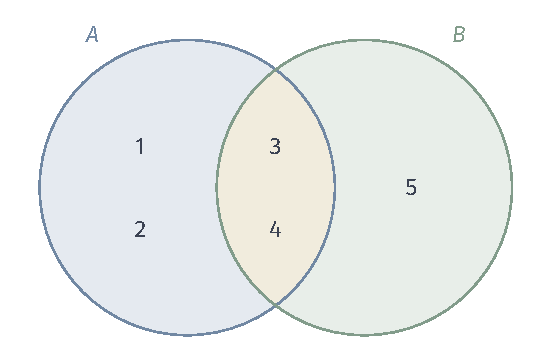
\includegraphics[width=90mm]{figures/01-mathematical-preliminaries-upper/01-mathematical-language-combinatorics-analysis-optimization/tikz/inclusion-exclusion-overlap.pdf}
  \caption{两个有限集合的重叠计数。$A=\{1,2,3,4\}$，$B=\{3,4,5\}$；仅属于$A$的区域放入$1,2$，公共区域放入$3,4$，仅属于$B$的区域放入$5$。把两圈元素个数相加时，公共区域被数两次，减去一次后得到并集中的五个不同元素。}
  \label{fig:comb-inclusion-exclusion-overlap}
\end{figure}

对三个集合逐元素检查：恰属于两个集合的元素先计两次、再减一次；同属三者的元素先计三次、减三次，还需加回一次。所以
\[
 |A\cup B\cup C|=|A|+|B|+|C|-|A\cap B|-|A\cap C|-|B\cap C|+|A\cap B\cap C|.
\]
\term{容斥原理}（inclusion--exclusion principle）把这种交替加减推广到任意有限个集合。
\begin{theorem}[有限容斥原理]
\label{thm:comb-inclusion-exclusion}
设$A_1,\ldots,A_m$是有限集合。则
\begin{equation}
  \Bigl|\bigcup_{i=1}^{m}A_i\Bigr|
  =\sum_{\varnothing\neq I\subseteq\{1,\ldots,m\}}(-1)^{|I|+1}\Bigl|\bigcap_{i\in I}A_i\Bigr|.
  \label{eq:comb-inclusion-exclusion}
\end{equation}
\end{theorem}
\begin{proof}
左侧每个并集元素恰计一次。右侧按元素合并，只需检查每个元素$x$的总系数。
设$x$恰属于$r$个集合，其下标组成$J$；$x$属于$\bigcap_{i\in I}A_i$当且仅当$I\subseteq J$。
$r=0$时$x$不在并集中，两侧都不计入。$r\geq1$时，大小为$k$的$I\subseteq J$有$\binom rk$个，所以$x$的总系数为
\[
 \sum_{k=1}^r(-1)^{k+1}\binom rk=-\Bigl(\sum_{k=0}^r(-1)^k\binom rk-1\Bigr)=1,
\]
最后一步用式~\eqref{eq:comb-alternating-subset-count}。所以两侧相等。
\end{proof}

\paragraph{补集计数}
有多条限制时，可以先数违反限制的结果，再从总数中减去。四门课的选法记作$\bm z=(z_1,z_2,z_3,z_4)\in\{0,1\}^4$，$z_i=1$表示选第$i$门。
规则是：课程$1,2$恰选一门；选课程$3$就必须选课程$1$；选课程$4$就必须在课程$2,3$中至少选一门。违反各条规则的选法分别组成
\[
 \begin{aligned}
 A_1&=\{\bm z:z_1=z_2\},\\
 A_2&=\{\bm z:z_3=1,\ z_1=0\},\\
 A_3&=\{\bm z:z_4=1,\ z_2=z_3=0\}.
 \end{aligned}
\]
由De Morgan律，合法选法组成$(A_1\cup A_2\cup A_3)^{\mathrm c}$，个数为$16-|A_1\cup A_2\cup A_3|$。
用乘法规则读出$|A_1|=8$、$|A_2|=4$、$|A_3|=2$；$A_1\cap A_2$要求$z_1=z_2=0$、$z_3=1$，有$2$个元素；
$A_1\cap A_3$只含$(0,0,0,1)$；$A_2\cap A_3$要求$z_3$既为$1$又为$0$，是空集。
由容斥原理，违规选法有$8+4+2-2-1-0+0=11$种，合法选法为$5$种，对应的课程集合族是
\begin{equation}
 \mathcal C_0=\bigl\{\{1\},\{1,3\},\{1,3,4\},\{2\},\{2,4\}\bigr\}.
 \label{eq:comb-running-feasible-family}
\end{equation}
直接分支计数也得到同样的五种：$z_1=1$时$z_3$任取、$z_4=1$须$z_3=1$，共三种；$z_2=1$时$z_3=0$、$z_4$任取，共两种。

\paragraph{递推计数}
固定元素$n$，把$V$的$k$元子集分成不含$n$与含$n$两类，分别有$\binom{n-1}k$与$\binom{n-1}{k-1}$个，所以
\[
 \binom nk=\binom{n-1}k+\binom{n-1}{k-1},\qquad n\geq1,
\]
称为Pascal恒等式。把它当作递推：令$a_{0,0}=1$，$0\leq k\leq n$以外的$a_{n,k}=0$，并对$n\geq1$规定
\begin{equation}
 a_{n,k}=a_{n-1,k}+a_{n-1,k-1}.
 \label{eq:comb-binomial-recurrence}
\end{equation}
逐行得到$(1)$、$(1,1)$、$(1,2,1)$、$(1,3,3,1)$、$(1,4,6,4,1)$；越界值取零使两端也适用同一规则。
对$n$归纳，并用Pascal恒等式与越界约定，可知$a_{n,k}=\binom nk$。图~\ref{fig:vol1-add-pascal-recurrence}标出了$\binom42=3+3$的来源。
\begin{figure}[!htb]
  \centering
  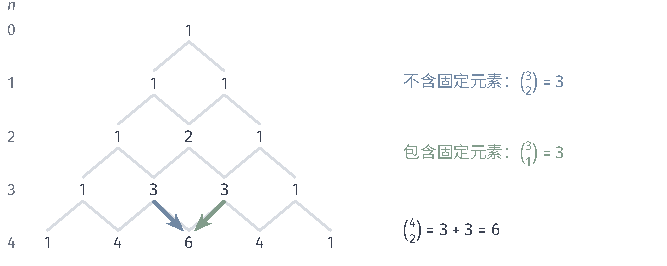
\includegraphics[width=112mm]{figures/01-mathematical-preliminaries-upper/00-shared/tikz/mathematical-language-combinatorics-analysis-optimization-comprehension-additions/pascal-recurrence.pdf}
  \caption{组合数的逐行递推。第$n$行列出$\binom n0,\ldots,\binom nn$；箭头突出$\binom42=\binom32+\binom31=3+3$。两种分类分别从其余三个元素选两个，或先保留固定元素再从其余三个中选一个。网格位置表示递推依赖，不表示子集包含关系。}
  \label{fig:vol1-add-pascal-recurrence}
\end{figure}

一般地，按固定元素、规模或最后一步分类，使每类成为更小的同类问题，就能建立递推。
例如长度为$n$、不含相邻两个$1$的零一记录个数$f_n$：按最后一位分类，末位为$0$时前$n-1$位任意合格，
末位为$1$时倒数第二位须为$0$、前$n-2$位任意合格，所以$f_n=f_{n-1}+f_{n-2}$（$n\geq2$），$f_0=1$、$f_1=2$。
递推式须与初值、适用范围一起写明。由各子集的累计值恢复其自身贡献的Möbius反演，放在图部分第~\ref{sec:comb-cumulative-inversion}节。

\section{本章小结}
\label{sec:comb-summary}

计数先确定什么算一个结果：是否区分次序、是否允许重复、各部分是否有名称。双射把难数的集合换成好数的集合；
互斥类别用加法，抽屉原理是其推论；各步选项数固定时用乘法，否则先分类再相加。
每个结果被记录同样多次时，记录数等于结果数乘以重复次数，排列数、组合数与二分划分的公式都由此得到；
允许重复的无序选择要先换成星号与竖线的记录。双重计数给出组合数之和，增删固定元素的配对给出交错和。
类别重叠时，容斥原理使每个元素恰计一次，补集计数借助De Morgan律把“满足全部限制”改写为“不违反任何一条”；
按固定元素、规模或最后一步分类可以建立递推。

这些方法依赖有限集合能被编号到某个$n$为止。对数不到最后一个元素的无限集合，
仍可以问两个集合的元素能否一一配对；第~\ref{chap:cardinality}章用双射和单射回答这一问题。

\chapter{基数}
\label{chap:cardinality}

正整数与正偶数，哪一个更多？正偶数只是正整数的一部分，似乎更少；
可是给每个正整数$n$配上正偶数$2n$，两边的元素又恰好一一配完。
有理数在数轴上处处稠密，实数是不是只比它“多一点”？
无限集合数不到最后一个元素，但有限集合的元素个数本来就由与$\{1,\ldots,n\}$的双射确定。
本章把“能否一一配对”当作比较大小的标准，推广到任意集合。

本章先用双射定义等势与基数，再用单射比较基数大小，证明两个方向的单射足以推出等势、幂集总严格更大；
最后研究可数集，整理可数性在哪些构造下保持，并证明有理数可数而实数不可数。
例子中用到读者熟悉的数系及其十进制表示，实数的确界与完备性在第~\ref{chap:function-limits}章建立。

\section{等势与基数的定义}
\label{sec:comb-cardinality}
\label{sec:comb-equinumerosity-cardinality}

\paragraph{等势与基数}
对任意两个集合，即使数不出个数，也可以问能否把两边的元素恰好一一配完。若存在双射$f:A\to B$，就称集合$A$与$B$\term{等势}（equinumerous）。
等势具有三条性质：恒等映射$\operatorname{id}_A$说明$A$与自身等势（自反）；
双射的逆映射仍是双射，所以$A$与$B$等势时$B$与$A$也等势（对称）；双射的复合仍是双射，
所以$A$与$B$、$B$与$C$等势时$A$与$C$等势（传递）。
等势只看能否配对，不依赖元素的名称：把$\{1,2,3\}$的元素改名为$a,b,c$，改名映射本身就是双射。

等势的集合称为具有相同的\term{基数}（cardinality），记作$|A|=|B|$。
$|A|=|B|$恰好意味着$A$与$B$等势；本章只用这一记号表达比较，不构造基数本身。

\paragraph{有限集合与无限集合的基数}
若$A$与某个$\{1,\ldots,n\}$等势（$n\geq0$），就称$A$为有限集合，它的基数沿用上一章的元素个数，$|A|=n$；
上一章已说明这样的$n$唯一，并约定$|\varnothing|=0$。与任何$\{1,\ldots,n\}$都不等势的集合称为无限集合。
例如$\mathbb N_+$是无限集合：若有双射$\{1,\ldots,n\}\to\mathbb N_+$，它的$n$个值中最大者加$1$不会被取到，与满射矛盾。

有限集合的真子集元素总是更少，上一章已由加法规则得到$B\subsetneq A$时$|A|>|B|$。无限集合却可能与自己的真子集等势。
映射$n\mapsto2n$从$\mathbb N_+$到正偶数集合是双射：不同的$n$给出不同的$2n$，每个正偶数$2m$都由$m$得到。
所以正偶数集虽是$\mathbb N_+$的真子集，基数却与$\mathbb N_+$相同。
可见“删去一部分元素后必定变少”不能搬到无限集合上，比较无限集合的大小只能依靠映射。
基数只记录元素的多少，不记录排列次序、几何位置或通常的长度。

\section{基数的性质}
\label{sec:comb-cardinality-properties}

等势只回答“是否一样多”。本节用单射定义“不超过”，并讨论两个方向的“不超过”能否推出一样多，以及是否存在最大的基数。

\paragraph{基于单射的比较}
若存在单射$f:A\to B$，$A$的每个元素都能占据$B$中一个不同的位置，这时记$|A|\leq|B|$。
若$|A|\leq|B|$但$A$与$B$不等势，记$|A|<|B|$。

双射是单射，所以等势的集合在两个方向上都满足$\leq$。

单射的复合仍是单射，所以$|A|\leq|B|$与$|B|\leq|C|$推出$|A|\leq|C|$，这种比较具有传递性。

若$A\subseteq B$，包含映射$a\mapsto a$是单射，所以子集的基数不超过原集合。

但真包含$A\subsetneq B$并不能推出$|A|<|B|$，正偶数集就是例子：要证明严格不等式，必须排除一切可能的双射。

\paragraph{双向单射推出等势}
若两个方向各有一个单射，两个集合是否一定一样多？对有限集合，比较元素个数即可得到肯定的回答；
对无限集合，两个单射各管一个方向，并不能直接拼成双射，需要另行构造。
\begin{theorem}[Cantor--Schröder--Bernstein定理]
\label{thm:comb-cantor-schroeder-bernstein}
若存在单射$f:A\to B$与$g:B\to A$，则存在双射$h:A\to B$，即$|A|=|B|$。
\end{theorem}
\begin{proof}
我们要为每个$a\in A$选定一个$B$中的配对对象，可选的只有两种：用$f$送到$f(a)$，或者在$a=g(b)$时沿$g$反向找回$b$。
不在$g(B)$中的元素没有反向对象，只能用$f$。设$a$用了$f$，那么$f(a)$已被占用，
元素$g(f(a))$就不能再反向找回$f(a)$，也只能用$f$；如此连锁下去。据此，
令$A_0=A\setminus g(B)$，并递推地令$A_{n+1}=g(f(A_n))$，即对$A_n$先施行$f$再施行$g$；
记$C=\bigcup_{n\geq0}A_n$，它收集了所有“只能用$f$”的元素，其余元素则用$g$的反向对应。定义$h:A\to B$：对$a\in C$令$h(a)=f(a)$；
对$a\in A\setminus C$，令$h(a)$为满足$g(b)=a$的那个$b$。
后一种规定有意义：$A_0\subseteq C$，所以$a\notin C$蕴含$a\notin A_0$，即$a\in g(B)$，这样的$b$存在；
又因为$g$是单射，它唯一。于是在$A\setminus C$上，$h$就是$g$的反向对应，满足$g(h(a))=a$。

下面验证$h$是双射。先看两块的像互不重叠：若某个$a\in C$与$a'\in A\setminus C$有$f(a)=h(a')$，
则$a'=g(h(a'))=g(f(a))$；而$a\in A_n$对某个$n$成立，于是$a'\in g(f(A_n))=A_{n+1}\subseteq C$，与$a'\notin C$矛盾。
再看每一块内部：$f$是单射，所以$h$在$C$上单射；在$A\setminus C$上，$h(a)=h(a')$两边作用$g$得$a=a'$。
两块内部单射且像不重叠，所以$h$是单射。最后看两块的像覆盖$B$：任取$b\in B$，若$g(b)\notin C$，
则$g(b)\in A\setminus C$，$h(g(b))$是满足$g(b')=g(b)$的$b'$，由$g$单射即$b$本身；
若$g(b)\in C$，由于$g(b)\in g(B)$，它不在$A_0$中，于是$g(b)\in A_{n+1}=g(f(A_n))$对某个$n$成立，
即存在$a\in A_n$使$g(b)=g(f(a))$，由$g$单射得$b=f(a)=h(a)$。所以$h$是满射，从而是双射。
\end{proof}
这一定理说明单射比较具有反对称性；连同自反性与传递性，基数的“不超过”在形式上与偏序相同。
证明两个集合等势时，只需在两个方向上各给一个单射，不必直接写出双射。

下面用这一方法证明区间$(0,1)$与实轴$\mathbb R$等势。一个方向，包含映射是$(0,1)$到$\mathbb R$的单射。

另一个方向，取
\[
 \varphi(x)=\frac12+\frac{x}{2(1+|x|)},\qquad x\in\mathbb R,
\]
需要验证两点。
\begin{itemize}
 \item 取值范围：由$|x|<1+|x|$得$\bigl|\frac{x}{2(1+|x|)}\bigr|<\frac12$，所以$\varphi(x)\in(0,1)$。
 \item 单射性：$\varphi(x)-\frac12$与$x$同号，所以$\varphi(x)=\varphi(y)$时$x,y$同号或同为零。
       若$x,y\geq0$，由$\frac{x}{1+x}=\frac{y}{1+y}$交叉相乘得$x=y$；若$x,y<0$，由$\frac{x}{1-x}=\frac{y}{1-y}$同样得$x=y$。
\end{itemize}
于是$\varphi$是$\mathbb R$到$(0,1)$的单射。

由Cantor--Schröder--Bernstein定理，$(0,1)$与$\mathbb R$等势。

长度为$1$的区间与整条实轴一样多，可见基数不反映长度。

\paragraph{幂集总有更大的基数}
有限集合满足$|\mathcal P(A)|=2^{|A|}>|A|$。对任意集合，这一严格不等式仍然成立。
\begin{theorem}[Cantor定理]
\label{thm:comb-cantor-power-set}
对任意集合$A$，都有$|A|<|\mathcal P(A)|$。
\end{theorem}
\begin{proof}
映射$a\mapsto\{a\}$把不同的元素送到不同的单元素集，是$A$到$\mathcal P(A)$的单射，所以$|A|\leq|\mathcal P(A)|$。
再设$f:A\to\mathcal P(A)$是任一映射，每个$f(a)$都是$A$的子集，可以问$a$本身是否属于它。构造
\[
 D=\{a\in A:a\notin f(a)\}\in\mathcal P(A).
\]
若$f$是满射，则存在$d\in A$使$f(d)=D$。按$D$的成员条件，$d\in D$当且仅当$d\notin f(d)$，
而$f(d)=D$，这就是说$d\in D$当且仅当$d\notin D$：若$d\in D$，则$d\notin D$；若$d\notin D$，则$d\in D$，两种情形都矛盾。
所以任何$f$都不是满射，更不是双射，结合前面的单射便得$|A|<|\mathcal P(A)|$。
\end{proof}
证明的关键是$D$的构造：对每个$a$，$D$与$f(a)$至少在元素$a$上不同，因为$a$恰好属于二者之一，
所以$D$不可能等于任何$f(a)$。这种逐个对象制造差异的构造称为对角线方法，后面证明实数不可数时还会用到。

上一章用零一记录数出了有限集合的子集个数。对任意集合，同样的对应仍然成立：每个子集$S\subseteq A$可由它的成员记录表示，
即$a\in S$时取$1$、否则取$0$的映射$\chi_S:A\to\{0,1\}$；反过来，每个映射$z:A\to\{0,1\}$都是子集$z^{-1}(\{1\})$的成员记录。
所以$S\mapsto\chi_S$是$\mathcal P(A)$到$\{0,1\}^A$（$A$到$\{0,1\}$的全部映射）的双射，二者等势。
有限情形下$|\{0,1\}^A|=2^{|A|}$；对无限集合，记号$2^{|A|}$就表示$\{0,1\}^A$的基数，也就是幂集的基数。

对任一集合反复取幂集，得到$A,\mathcal P(A),\mathcal P(\mathcal P(A)),\ldots$，基数一个比一个大。
所以不存在最大的基数：任给一个集合，它的幂集都更大。这一结论只讨论任意给定的集合及其幂集，
不把“所有集合”当作一个集合；若把全部集合收集成一个集合$V$，幂集$\mathcal P(V)$的元素都是集合，因而$\mathcal P(V)\subseteq V$，
基数不超过$V$，与Cantor定理矛盾。

\section{可数集}
\label{sec:comb-countable-sets}

能用正整数编号列尽的集合，是后文讨论数列、可数求和与可数覆盖的基础。
本节给出定义与列表刻画，整理可数性的保持规则，再说明有理数可数、实数和无限零一序列不可数。

\subsection{可数集的定义}
\label{sec:countable-set-definition}

\begin{definition}[可数集]
\label{def:analysis-countable-set}
能与正整数集$\mathbb N_+$等势的集合称为可数无限集。
有限集与可数无限集统称\term{可数集}（countable set）；不是可数集的集合称为\term{不可数集}（uncountable set）。
\end{definition}
可数无限集的基数记为$\aleph_0$，读作“阿列夫零”；有限集也算可数集，但其基数是非负整数。
由等势的对称性与传递性，与可数集等势的集合仍可数，与不可数集等势的集合仍不可数。

按定义证明可数，需要写出没有重复的编号；实际构造时，往往只能先写出一个可能有重复的列表。
下面的定理说明，只要列表不遗漏元素，重复并无妨碍。
\begin{theorem}[可数集的列表刻画]
\label{thm:comb-countable-surjection}
非空集合$A$可数，当且仅当存在满射$g:\mathbb N_+\to A$。
\end{theorem}
\begin{proof}
若$A$是可数无限集，取双射$g:\mathbb N_+\to A$即可。若$A=\{a_1,\ldots,a_m\}$有限且$m\geq1$，
令$n\leq m$时$g(n)=a_n$、$n>m$时$g(n)=a_m$，即重复末项把有限列表延长，它是满射。
反之，设$g$是满射。沿$n=1,2,\ldots$依次检查$g(n)$，只保留此前未出现过的值，即按首次出现去重。
每个$a\in A$都等于某个$g(n)$，因而在第$n$步或更早被保留；保留下来的元素互不相同。
若保留的元素只有有限个，$A$是有限集；否则按保留的先后编号$1,2,\ldots$，得到$\mathbb N_+$与$A$的双射。
\end{proof}
于是，要证明一个非空集合可数，只需给出一个可以有重复、但不遗漏任何元素的列表。
空集没有这样的列表，但它是有限集，本身可数，以下各结论中都单独处理。

\subsection{可数集的性质}
\label{sec:countable-set-properties}

\paragraph{子集与函数的像}
由列表刻画，删去一部分元素或用映射把元素送到另一个集合，都不会把可数集变成不可数集。
\begin{theorem}[子集与像的可数性]
\label{thm:comb-countable-subset-image}
设$A$可数。则$A$的每个子集可数；对任意映射$f:A\to Y$，像$f(A)$可数。
特别地，若存在单射$h:B\to\mathbb N_+$，则$B$可数。
\end{theorem}
\begin{proof}
空集以及$A=\varnothing$时的像$f(\varnothing)=\varnothing$都可数，以下设$A$非空，取满射$g:\mathbb N_+\to A$。
对像，逐项取像得到列表$f(g(1)),f(g(2)),\ldots$，即$f\circ g:\mathbb N_+\to f(A)$，它仍是满射，由列表刻画$f(A)$可数。
对非空子集$E\subseteq A$，取定$e_0\in E$，把列表中不属于$E$的项都换成$e_0$，即定义$r(a)=a$（$a\in E$）、$r(a)=e_0$（$a\notin E$）；
$r:A\to E$是满射，所以$E=r(A)$是可数集的像，因而可数。
最后，单射$h$给出$B$与$h(B)$之间的双射，而$h(B)\subseteq\mathbb N_+$可数，故$B$可数。
\end{proof}
例如素数集可数。最后一条是常用判据：给$B$的元素指定互不相同的正整数编码，$B$就可数。

\paragraph{有限笛卡尔积}
怎样列出全部正整数对？若逐行列举$\mathbb N_+^2$，就会在第一行$(1,1),(1,2),\ldots$永远进行下去，到不了第二行。
改按坐标和由小到大分层列举：先$(1,1)$，再$(1,2),(2,1)$，再$(1,3),(2,2),(3,1)$，依此类推。
坐标和为$s$的一层只有$s-1$项，所以每层有限；任意一对$(i,j)$都在坐标和为$i+j$的那一层出现，且只出现一次。
因此这份列表在有限步内到达每一对，给出$\mathbb N_+$与$\mathbb N_+^2$的双射，正整数对的集合可数。
借助这份列表，可以处理任意有限个可数集的乘积。
\begin{theorem}[有限笛卡尔积的可数性]
\label{thm:comb-countable-product}
若$A_1,\ldots,A_k$可数，则$A_1\times\cdots\times A_k$可数。
\end{theorem}
\begin{proof}
若某个$A_i$为空，乘积为空集，结论成立。以下设各$A_i$非空，对$k$归纳，$k=1$时无需证明。
设$P=A_1\times\cdots\times A_k$可数；它非空，可取满射$g:\mathbb N_+\to P$与$g':\mathbb N_+\to A_{k+1}$。
映射$(m,n)\mapsto(g(m),g'(n))$是$\mathbb N_+^2$到$P\times A_{k+1}$的满射，
所以$P\times A_{k+1}$是可数集$\mathbb N_+^2$的像，由定理~\ref{thm:comb-countable-subset-image}可数；
它与$A_1\times\cdots\times A_{k+1}$之间有双射，故后者也可数。
\end{proof}
例如$\mathbb N^d$对每个正整数$d$都可数。

\paragraph{可数个可数集的并}
若有可数多组对象，每组都能列举，能否给合并后的全部对象统一编号？
\begin{theorem}[可数并的可数性]
\label{thm:comb-countable-union}
设$(A_n)_{n\in\mathbb N_+}$中每个$A_n$可数，并且对每个非空的$A_n$已给定一个满射$g_n:\mathbb N_+\to A_n$。
则$\bigcup_{n\in\mathbb N_+}A_n$可数。
\end{theorem}
\begin{proof}
设$I=\{n:A_n\neq\varnothing\}$，若$I$为空则并集为空。否则$I$作为$\mathbb N_+$的子集可数，
$I\times\mathbb N_+$由定理~\ref{thm:comb-countable-product}可数。映射$(n,j)\mapsto g_n(j)$是$I\times\mathbb N_+$到
$\bigcup_nA_n$的满射：并集中的每个元素属于某个非空$A_n$，又是$g_n$的某个值。由定理~\ref{thm:comb-countable-subset-image}，并集可数。
\end{proof}
证明相当于把双索引的全部$g_n(j)$按$(n,j)$的坐标和分层列出，重复出现的元素只保留第一次。
同一元素可以属于多个$A_n$，也可以在同一个列表中多次出现；这些重复只影响编号，不影响可数性。
定理要求事先给定各组的列表，本书遇到的可数并都带有明确的列表。
有限个可数集的并也包括在内，只需令其余的$A_n$为空集。
例如，全部有限长度的自然数序列组成的集合可数：长度为$k\geq1$的序列组成$\mathbb N^k$，由有限积的结论可数，
并且可以按前面的分层方式写出列表；长度为$0$的只有空序列。全部有限长度序列是这些集合对$k=0,1,2,\ldots$的并，所以仍可数。

\paragraph{有理数的可数性}
有理数在数轴上稠密：任意两个不同有理数之间还有无限多个有理数，似乎无法逐个列出。上面的保持规则却说明它们可以列尽。
\begin{theorem}[有理数可数]
\label{thm:card-rationals-countable}
整数集$\mathbb Z$与有理数集$\mathbb Q$都是可数集，$|\mathbb Z|=|\mathbb Q|=\aleph_0$。
\end{theorem}
\begin{proof}
把整数排成$z_1,z_2,z_3,\ldots=0,1,-1,2,-2,\ldots$，即第$2k$项是$k$、第$2k+1$项是$-k$；每个整数恰好出现一次，所以$\mathbb Z$是可数无限集。
每个有理数都能写成$p/q$，其中$p\in\mathbb Z$、$q\in\mathbb N_+$，所以$\mathbb Q$是$\mathbb Z\times\mathbb N_+$在映射$(p,q)\mapsto p/q$下的像。
由有限笛卡尔积与像的可数性，$\mathbb Q$可数；又因为$\mathbb Q\supseteq\mathbb N_+$不是有限集，它是可数无限集。
\end{proof}
证明中的列表可以具体写出：按正整数对$(i,j)$的坐标和分层，依次写出$z_i/j$，得到
\[
 \frac{0}{1},\ \frac{0}{2},\ \frac{1}{1},\ \frac{0}{3},\ \frac{1}{2},\ \frac{-1}{1},\ \ldots.
\]
列表有重复，例如$0/1$与$0/2$表示同一个有理数；按列表刻画，只保留每个有理数首次出现的位置，就得到$\mathbb N_+$与$\mathbb Q$的双射。
同理$\mathbb Q^d$可数，即坐标全为有理数的点在$\mathbb R^d$中只有可数多个。稠密与可数互不妨碍。

\paragraph{实数的不可数性}
\phantomsection
\label{sec:comb-real-uncountable}
有理数能被列尽，实数却不能。证明用到读者已有的十进制表示知识：每个实数都有十进制表示，
同一实数有两种表示只发生在以全$0$与全$9$结尾的情形，例如$0.5000\cdots=0.4999\cdots$；
这些事实依赖实数的完备性（第~\ref{chap:function-limits}章的确界原理），本章不展开其证明。
\begin{theorem}[实数不可数]
\label{thm:card-reals-uncountable}
开区间$(0,1)$与实数集$\mathbb R$都是不可数集。
\end{theorem}
\begin{proof}
$(0,1)$含有全部$1/(n+1)$，不是有限集。假设它是可数无限集，其元素可以列为$x_1,x_2,\ldots$。
给每个$x_n$选定一个不以无限多个$9$结尾的十进制表示$x_n=0.d_{n,1}d_{n,2}d_{n,3}\cdots$，
构造$y=0.c_1c_2c_3\cdots$：若$d_{n,n}=1$就取$c_n=2$，否则取$c_n=1$。则$y\in(0,1)$，并且对每个$n$，$y$的第$n$位与$x_n$的第$n$位不同。
$y$只用数字$1,2$，其表示唯一；$x_n$的表示也不以全$9$结尾。所以第$n$位不同意味着$y\neq x_n$，$y$不在列表中，矛盾。
因此$(0,1)$不可数。若$\mathbb R$可数，由子集的可数性，$(0,1)$也可数，矛盾，所以$\mathbb R$不可数。
\end{proof}

实数集的基数记为$\mathfrak c$，称为连续统的基数（cardinality of the continuum）。
对端点$a<b$的任一区间$I$，一方面$I\subseteq\mathbb R$；另一方面线性映射$t\mapsto a+(b-a)t$把$(0,1)$双射到$(a,b)\subseteq I$，
与单射$\varphi:\mathbb R\to(0,1)$复合得到$\mathbb R$到$I$的单射。由Cantor--Schröder--Bernstein定理，$|I|=\mathfrak c$：
长度不同的区间仍一样多。又因为$\mathbb N_+\subseteq\mathbb R$而$\mathbb R$不可数，有$\aleph_0<\mathfrak c$。

\paragraph{无理数的不可数性}
有理数可数而实数不可数，二者之差的无理数便不可能只有可数多个。
\begin{theorem}[无理数不可数]
\label{thm:card-irrationals-uncountable}
无理数集$\mathbb R\setminus\mathbb Q$是不可数集。
\end{theorem}
\begin{proof}
假设$\mathbb R\setminus\mathbb Q$可数。由定理~\ref{thm:card-rationals-countable}，$\mathbb Q$可数，
于是$\mathbb R=\mathbb Q\cup(\mathbb R\setminus\mathbb Q)$是两个可数集的并，由可数并的可数性（取其余$A_n$为空集）可数，
与定理~\ref{thm:card-reals-uncountable}矛盾。
\end{proof}
证明也说明，不可数集不能由可数多个可数集拼成。

\paragraph{幂集与无限序列的不可数性}
\phantomsection
\label{sec:comb-uncountable-power-set}
回看Cantor定理：$\mathcal P(\mathbb N_+)$不是有限集，又由$|\mathbb N_+|<|\mathcal P(\mathbb N_+)|$不与$\mathbb N_+$等势，所以不可数；
经成员记录，全部无限零一序列组成的$\{0,1\}^{\mathbb N_+}$与它等势，也不可数。
这与实数的证明是同一种对角线构造：$D$在元素$a$上与$f(a)$不同，$y$在第$n$位上与$x_n$不同。
$\{0,1\}^{\mathbb N_+}$可以看成可数多个两元集的笛卡尔积，所以有限积、可数并保持可数性，并不意味着无限积也保持可数性。

\section{本章小结}
\label{sec:cardinality-summary}

本章把“能否一一配对”作为比较集合大小的标准：双射定义等势与基数，单射定义“不超过”。
相应地，每一种映射构造给出一种结论。给出双射，就证明了等势；给出单射，就证明了不超过；
两个方向各给出一个单射，由Cantor--Schröder--Bernstein定理也能推出等势。
证明严格更大则要排除一切满射，Cantor定理用对角线构造做到了这一点，由此得出幂集总更大、不存在最大的基数。
无限集合可以与真子集等势，长度不同的区间也可以等势，所以基数不反映次序、位置或长度。

以正整数集为标准，可数集就是能被一个（允许重复的）列表列尽的集合。子集、映射的像、有限笛卡尔积与给定列举的可数并都保持可数性，
因此整数、正整数对、有限长度序列与有理数都可数；无限零一序列、正整数集的幂集与实数集则不可数，$\aleph_0<\mathfrak c$。
有理数稠密而可数，实数却不可数，说明数轴上“处处都有”与“能够编号”是两回事。
实数为什么有十进制表示，确界与极限为什么存在，都要从实数的完备性出发说明。
第~\ref{chap:function-limits}章从实值函数的确界开始，建立数列与函数的极限；后文讨论可数覆盖与可数求和时，还会反复用到本章的可数性规则。

\chapter{函数的极限}
\label{chap:function-limits}
\label{chap:mathematical-analysis}

第~\ref{chap:sets-functions-and-proofs}章末尾的等比递推$e^{(t)}=\rho^te_0$给出了有限步结果；
当$t$无限增大时，这些数是否趋向确定的值？有限几何和在项数增加时又怎样变化？
本章先用数列和函数的极限精确说明“趋近”，区分极限的计算与存在性判别，
再用部分和的极限建立级数，并检查重排与保序分组的不同条件。
极限定义通过距离控制误差，因此随后把实数的绝对值距离推广为度量，建立开集、闭集、完备性与紧致性。
这些认识为后续一元与多元微积分提供共同的极限语言。

\section{序列的极限}
\label{sec:analysis-continuous-limits}

数列$1,1/2,1/3,\ldots$越来越接近$0$，数列$-1,1,-1,1,\ldots$则在两个值之间来回交替。
直觉上前者“有极限”，后者没有；但“越来越接近”需要精确的含义，否则无法判断更复杂的情形，
例如$(1+1/n)^n$或$\sum_{k\leq n}1/k$是否趋向某个数。
极限用误差条件给出这种含义：给定任意小的误差，后面的项是否都能落在这一误差范围内。
本节先研究实数列，说明怎样计算极限、怎样在不知道极限值时保证极限存在；
再把数列极限用于不断增加项数的和，得到无穷级数。
下一节再研究函数输入趋近某点时函数值的趋向。

\label{sec:analysis-sequences-series-errors}

判断一列数是否趋近某个数，有两类问题：已知各列收敛时，怎样计算它们组合后的极限；
尚不知道极限时，怎样从数列本身的性质保证极限存在。前者可以借助夹逼与极限的运算法则，
后者依靠单调有界、收敛子列和柯西准则；这三种存在性判别都要用到第~\ref{chap:sets-functions-and-proofs}章的确界原理。
下面先定义收敛，再建立收敛判别，随后集中讨论极限的基本性质、运算与夹逼，最后将这些结论用于无穷级数。

\subsection{数列的收敛}

\paragraph{收敛与发散}
数列$(a_n)_{n\geq1}$是一列按正整数排列的实数。
例如$(1/n)$的项越来越接近$0$，而$((-1)^n)$在$-1$和$1$之间交替。
“接近一个数”要同时约束后面的全部项，不能只看某几个位置：$((-1)^n)$的偶数项都等于$1$，
但奇数项始终离$1$有距离$2$，所以它不应算作趋于$1$。
同样，只要求“各项与$a$的距离越来越小”也不够，例如$1+1/n$离$0$越来越近，却始终大于$1$。
合适的要求是：无论事先给定多小的正误差，从某一项起，后面\emph{每一项}与$a$的距离都小于这个误差。
若存在$a\in\mathbb R$，使每个$\varepsilon>0$都对应一个整数$N$，满足
\[
 n\geq N\quad\Longrightarrow\quad |a_n-a|<\varepsilon,
\]
就称$(a_n)$\term{收敛}（converge）到$a$，$a$称为其极限，记作
$\lim_{n\to\infty}a_n=a$或$a_n\to a$。没有有限实数极限时，称数列发散（diverge）。
这里先任给误差$\varepsilon$，再选取$N$；选定以后，所有$n\geq N$都须满足要求。
例如对$a_n=1/n$，任给$\varepsilon>0$，取整数$N>1/\varepsilon$，则$n\geq N$时
$|a_n-0|=1/n\leq1/N<\varepsilon$，所以$1/n\to0$。这样的整数$N$一定存在，因为正整数没有上界
（否则其上确界$s$会使$s-1$不是上界，存在正整数$k>s-1$，从而$k+1>s$，矛盾）。
$N$可以依赖于给定的$\varepsilon$；误差要求越严格，所需的尾部起点通常越靠后，定义不要求这个$N$唯一。
反过来，要说明$((-1)^n)$不收敛到任何$a$，只需取$\varepsilon=1$：
相邻两项相差$2$，不可能同时落在长度为$2$的开区间$(a-1,a+1)$内，所以没有$N$能使后面全部项满足要求。
极限不要求某一项恰好等于$a$\scite{math-lebl-analysis1}。


图~\ref{fig:analysis-process-sequence-tail}把“全部尾部项”画成同一条误差带：选定起点以后，后面每一项都必须留在带内。
\begin{figure}[!htbp]
 \centering
 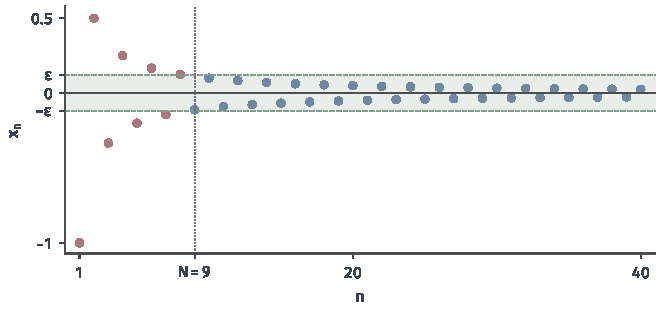
\includegraphics[width=112.0mm]{figures/01-mathematical-preliminaries-upper/01-mathematical-language-combinatorics-analysis-optimization/matplotlib/chapter3-concept-processes/sequence-tail.pdf}
 \caption{数列$x_n=(-1)^n/n$的前40项。绿色带为$|x_n|<0.12$，取$N=9$后，所有$n\geq9$都在带内；蓝点标记这个尾部，红点标记之前的项。尾部条件针对无限多个$n$，其成立依据是$1/n\leq1/9<0.12$，不是只检查图中有限个点。}
 \label{fig:analysis-process-sequence-tail}
\end{figure}

\subsection{数列的收敛判别}

定义收敛时需要指定一个候选极限，但很多数列的候选极限尚不明确。
下面依次利用变化方向、取值范围和尾部互近来判断极限是否存在，并说明各自需要的条件。

\subsubsection{单调数列的收敛}
若候选极限尚未确定，可以同时限制数列的变化方向和取值范围。
若对所有$n$都有$a_n\leq a_{n+1}$，称数列单调不减；
若总有$a_n\geq a_{n+1}$，称数列单调不增，两者统称为单调数列。

对于单调不减且有上界的数列，第~\ref{sec:prelim-optimal-values-errors}节的确界性质
为全部项提供一个最小上界；单调性将保证后面的项一直靠近它。
\begin{theorem}[单调有界收敛定理]
\label{thm:analysis-monotone-bounded-sequence}
设$(a_n)_{n\geq1}$为实数列。
若$a_n\leq a_{n+1}$对所有$n\geq1$成立，且存在$M\in\mathbb R$使$a_n\leq M$对所有$n\geq1$成立，则
\[
 \lim_{n\to\infty}a_n=\sup\{a_n:n\geq1\}\in\mathbb R.
\]
若$a_n\geq a_{n+1}$对所有$n\geq1$成立，且存在$m\in\mathbb R$使$a_n\geq m$对所有$n\geq1$成立，则
\[
 \lim_{n\to\infty}a_n=\inf\{a_n:n\geq1\}\in\mathbb R.
\]
\end{theorem}
\begin{proof}
设$a=\sup\{a_n:n\geq1\}$。给定$\varepsilon>0$，$a-\varepsilon$不是上界，
所以存在$N$使$a_N>a-\varepsilon$。单调性使$n\geq N$时都有
$a-\varepsilon<a_N\leq a_n\leq a$，这正是$a_n\to a$。
单调不增的情形对$-a_n$应用同一论证。
\end{proof}
这里使用实数\term{完备性}（completeness）的具体位置，是保证非空上有界实数集合的上确界仍为实数，
而不是另加一种数列变化条件。“有界”与“单调”也不能省去：$n$单调却无上界，
$(-1)^n$有界却不单调。

\subsubsection{有界数列的子序列收敛}
数列可能整体不收敛，但其中一些项仍有共同的趋向。保持原有次序选出一部分项，
得到子序列（subsequence），也称子列：若$n_1<n_2<\cdots$为严格递增的正整数列，
则$(a_{n_k})_{k\geq1}$为$(a_n)$的子序列。
收敛数列的每个子序列都收敛到同一极限，因为$n_k\to\infty$，原来的尾部误差界仍适用。
一个子序列收敛不能保证原数列收敛；$(-1)^n$的偶数项恒为$1$，奇数项恒为$-1$。

有界性不足以保证整列收敛，却能保证从中选出一个收敛子序列。
下面的结论称为Bolzano--Weierstrass定理，随后将用它证明柯西条件足以保证实数列收敛。
\begin{theorem}[Bolzano--Weierstrass定理]
\label{thm:analysis-bounded-subsequence}
设$(a_n)_{n\geq1}$为实数列。若存在$M\geq0$使$|a_n|\leq M$对所有$n\geq1$成立，
则存在严格递增的正整数列$n_1<n_2<\cdots$和$a\in\mathbb R$，使
\[
 \forall\varepsilon>0,\quad\exists K\in\{1,2,\ldots\},\quad
 k\geq K\Longrightarrow |a_{n_k}-a|<\varepsilon.
\]
即$a_{n_k}\to a$。
\end{theorem}
\begin{proof}
先取包含全部项的闭区间，将它平分，至少有一半仍包含无穷多项；
反复选择，得到嵌套闭区间$I_k=[l_k,r_k]$，每个区间都含无穷多项，长度为原长度的$2^{-k}$倍。
由$2^k\geq k+1$，这些长度至多为原长度的$1/(k+1)$，因而趋于零；这里不必先用后面的等比数列极限。
依次选取下标递增且$a_{n_k}\in I_k$的项。
由确界性质，$c=\sup_k l_k$满足$l_k\leq c\leq r_k$对每个$k$成立：
各$l_k$单调不减，而每个$r_k$都是所有左端点的上界。
给定$\varepsilon>0$，先选$K$使$r_K-l_K<\varepsilon$；
当$k\geq K$时，$a_{n_k}$与$c$同在$I_K$内，所以$|a_{n_k}-c|<\varepsilon$。
\end{proof}

\subsubsection{柯西数列的收敛}
单调条件并不适用于所有收敛数列。若还不知道候选极限，可以检查尾部各项是否彼此接近。
满足
\[
 \forall\varepsilon>0,\quad\exists N,\quad
 \forall m,n\geq N,\quad |a_m-a_n|<\varepsilon
\]
的数列称为\term{柯西数列}（Cauchy sequence）。
这个条件不指定候选极限，只比较尾部各项。对实数列，它与收敛等价。
\begin{theorem}[柯西收敛准则]
\label{thm:analysis-cauchy-convergence}
设$(a_n)_{n\geq1}$为实数列。存在$a\in\mathbb R$使$a_n\to a$，当且仅当
\[
 \forall\varepsilon>0,\quad\exists N\in\{1,2,\ldots\},\quad
 \forall m,n\geq N,\quad |a_m-a_n|<\varepsilon.
\]
\end{theorem}
\begin{proof}
每个收敛实数列都是柯西数列，因为
$|a_m-a_n|\leq|a_m-a|+|a_n-a|$，分别控制右侧两项即可。

反过来，柯西条件先保证数列有界：取误差$1$，尾部都在某一项两侧距离$1$以内，
有限个前项另取一个界即可。由上面的收敛子列结论，可取$a_{n_k}\to a$。
给定$\varepsilon>0$，先使任意$m,n\geq N$满足$|a_m-a_n|<\varepsilon/2$，
再选$n_k\geq N$使$|a_{n_k}-a|<\varepsilon/2$。
对每个$n\geq N$都有
$|a_n-a|\leq|a_n-a_{n_k}|+|a_{n_k}-a|<\varepsilon$。
\end{proof}
这一准则不必预先猜出极限；其充分性仍通过收敛子列依赖实数的确界性质。

验证柯西条件时，可把两个较晚的项之间的距离估计为逐步变化的总和。对$m>n$，
\begin{equation}
 |a_m-a_n|\leq\sum_{k=n}^{m-1}|a_{k+1}-a_k|.
\label{eq:analysis-cauchy-tail-bound}
\end{equation}
相邻差趋零还不够，因为中间的步数也在增加，必须控制整段和。
例如$a_1=0$、$a_{k+1}-a_k=1/k$时，每一步都趋零，但
$a_{2n}-a_n=\sum_{k=n}^{2n-1}1/k>1/2$，所以它不是柯西数列。
这一差别把极限问题引向下面的级数：单次贡献变小，并不等于全部贡献的累计稳定。

\subsection{极限的基本性质}

前面的判别给出了保证收敛的条件。现在假定实数列已经收敛，先检查极限的唯一性及数列的有界性，再分别计算和、差、数乘、积与商的极限，最后说明怎样用上下界夹逼求极限。
这些运算法则都以有限极限存在为前提，不能代替收敛性的判别。

\paragraph{极限的唯一性}
先假定极限存在，考察定义已经保证了什么。极限必唯一：若$a\neq b$都是极限，
取$\varepsilon=|a-b|/3$，充分靠后的项应同时满足
$|a_n-a|<\varepsilon$和$|a_n-b|<\varepsilon$；
三角不等式却给出$|a-b|\leq|a-a_n|+|a_n-b|<2|a-b|/3$，矛盾。

\paragraph{收敛数列的有界性}
收敛数列还必有界。取$\varepsilon=1$后，除有限个前项外都有$|a_n|\leq|a|+1$，
再把有限个前项的绝对值一并取最大值，即得到全列的界。
反向结论不成立，例如$(-1)^n$有界却不收敛；有界性只限制取值范围，没有控制尾部是否还在振荡。

\paragraph{和的极限}
实际计算时，一个数列常由几个已知数列相加得到。设$a_n\to a$、$b_n\to b$，其中$a,b\in\mathbb R$，则
\[
 \lim_{n\to\infty}(a_n+b_n)=a+b.
\]
因为$|(a_n+b_n)-(a+b)|\leq|a_n-a|+|b_n-b|$，
只需让两个误差分别小于$\varepsilon/2$，便能使和的误差小于$\varepsilon$。

\paragraph{差的极限}
相减时也可以分别控制两列数的误差。在同样的有限收敛条件下，
\[
 \lim_{n\to\infty}(a_n-b_n)=a-b.
\]
这来自$|(a_n-b_n)-(a-b)|\leq|a_n-a|+|b_n-b|$，取尾部起点使右侧两项各小于$\varepsilon/2$即可。

\paragraph{数乘的极限}
把每一项乘以固定的实数$c$，只会把误差乘以$|c|$，所以
\[
 \lim_{n\to\infty}ca_n=ca.
\]
$c=0$时结论直接成立；$c\neq0$时，把原数列误差控制在$\varepsilon/|c|$以内即可。

\paragraph{积的极限}
乘积的误差还包含一个变化的因子，因此先用收敛数列有界这一性质。若$a_n\to a$、$b_n\to b$，则
\[
 \lim_{n\to\infty}a_nb_n=ab.
\]
取$M\geq1$使所有$|a_n|\leq M$，分解误差得
\[
 |a_nb_n-ab|\leq M|b_n-b|+|b|\,|a_n-a|.
\]
让$|b_n-b|<\varepsilon/(2M)$、$|a_n-a|<\varepsilon/[2(|b|+1)]$同时成立，右侧便小于$\varepsilon$。

\paragraph{商的极限}
除法还须避免分母趋零。若$a_n\to a$、$b_n\to b$且$b\neq0$，则充分靠后的$b_n\neq0$，并且
\[
 \lim_{n\to\infty}\frac{a_n}{b_n}=\frac ab.
\]
事实上，充分靠后的$|b_n|\geq|b|/2$，于是
$|1/b_n-1/b|\leq2|b_n-b|/|b|^2\to0$，结合乘积规则即得结论。
例如将分子分母同除以$n$，可得$n/(n+1)\to1$。
这些运算法则针对已经存在的有限极限，不能把$0/0$或$\infty-\infty$直接当成数值计算。

\paragraph{夹逼定理}
有时中间数列不断振荡，直接控制它的误差并不方便，但可以分别找到上下界。
若上下两列最终都靠近同一有限值，中间数列便被限制在同一误差范围内。
\begin{theorem}[夹逼定理]
\label{thm:analysis-sequence-squeeze}
设$(a_n)$、$(b_n)$、$(c_n)$为实数列。若存在正整数$N_0$使
\[
 \forall n\geq N_0,\qquad a_n\leq c_n\leq b_n,
\]
并且存在$\ell\in\mathbb R$满足
$\lim_{n\to\infty}a_n=\lim_{n\to\infty}b_n=\ell$，则
$\lim_{n\to\infty}c_n=\ell$。
\end{theorem}
\begin{proof}
任给$\varepsilon>0$，由两端收敛可选正整数$N_1,N_2$，使
$n\geq N_1$时$|a_n-\ell|<\varepsilon$，$n\geq N_2$时$|b_n-\ell|<\varepsilon$。
取$N=\max\{N_0,N_1,N_2\}$，则每个$n\geq N$都有
\[
 \ell-\varepsilon<a_n\leq c_n\leq b_n<\ell+\varepsilon.
\]
所以$|c_n-\ell|<\varepsilon$，按定义即$c_n\to\ell$。
\end{proof}
例如$-1/n\leq(\sin n)/n\leq1/n$，所以$(\sin n)/n\to0$。

一个反复使用的例子是$|r|<1$时$r^n\to0$。$r=0$时直接成立；
若$0<|r|<1$，写$1/|r|=1+h$，其中$h>0$。
从$(1+h)^1=1+h$出发，每多乘一次$1+h$，都有
$(1+nh)(1+h)\geq1+(n+1)h$，所以$(1+h)^n\geq1+nh$。
因此$0<|r|^n\leq1/(1+nh)\to0$，再由夹逼定理得到结论。
这也给出式~\eqref{eq:prelim-geometric-recurrence}所定义等比递推的极限。

\subsection{数列的上极限与下极限}
有些数列既不收敛，也没有柯西性质；仍可考察它们尾部的上下边界。
为记录无界的趋向，约定$a_n\to+\infty$表示对每个实数$M$，充分大的$n$都满足$a_n>M$；
$a_n\to-\infty$则要求最终都有$a_n<M$。
这两个符号不是有限实数极限，$\overline{\mathbb R}=\mathbb R\cup\{-\infty,+\infty\}$称为扩展实数，
其中$\infty-\infty$没有定义。

逐渐舍去前项时，尾部下界只会上升，尾部上界只会下降，因此可以分别用单调极限记录它们。
\begin{definition}[数列的上极限与下极限]
\label{def:analysis-liminf-limsup}
对扩展实数列$(a_n)$，定义
\[
 \liminf_{n\to\infty}a_n
 =\lim_{n\to\infty}\inf_{k\geq n}a_k,
 \qquad
 \limsup_{n\to\infty}a_n
 =\lim_{n\to\infty}\sup_{k\geq n}a_k.
\]
右侧尾部下确界随$n$单调不减，尾部上确界随$n$单调不增，故两者的极限均在扩展实数中存在。
\end{definition}
例如$(-1)^n$的下极限为$-1$、上极限为$1$，通常极限不存在。
总有$\liminf a_n\leq\limsup a_n$；二者同为有限$a$当且仅当$a_n\to a$，
因为此时充分靠后的尾部上下边界可同时落在$a$附近，夹逼便控制了每个尾部项。
二者同为$+\infty$或$-\infty$时则对应上述无穷极限，仍应与有限实数收敛区别。
对有界实数列，上、下极限还是能够由子序列达到的极限：例如记$L=\limsup a_n$，
在足够晚的尾部内选一项大于$L-1/j$，并要求其下标超过前次所选的下标；
尾部上界又最终小于$L+1/j$，由此可构造趋于$L$的子列，下极限同理。

\subsection{级数的收敛}

\paragraph{级数与部分和}
把有限和的上限不断增大，就得到新的数列
\[
 s_N=\sum_{n=1}^{N}a_n=a_1+\cdots+a_N,
\]
$s_N$称为\term{部分和}（partial sum）。
符号\term{无穷级数}（infinite series）$\sum_{n=1}^{\infty}a_n$描述这一求和过程；
当$(s_N)$有有限极限$s$时，称级数收敛，并记$\sum_{n=1}^{\infty}a_n=s$。
例如$a_n=2^{-n}\to0$，但部分和$s_N=1-2^{-N}\to1$；
单项极限与级数的和是两个不同的对象。
由$a_N=s_N-s_{N-1}$可知，级数收敛必须有$a_N\to0$，反向则不成立，下面的$p=1$就是反例。

若所有$a_n\geq0$，部分和单调不减，因此有界时收敛，无界时趋于$+\infty$。
这种情形下统一记
\[
 \sum_{n=1}^{\infty}a_n:=\sup_N\sum_{n=1}^{N}a_n\in[0,+\infty].
\]
这是非负项级数的扩展总和；总和为$+\infty$时仍称级数发散，不把它混同于有限和。
非负项的累计没有正负抵消，因而可以直接比较不同部分和的大小。

\paragraph{几何级数}
第~\ref{chap:sets-functions-and-proofs}章的有限几何和公式~\eqref{eq:prelim-finite-geometric-sum}给出$r\neq1$时
\[
 \sum_{n=0}^{N}r^n=\frac{1-r^{N+1}}{1-r}.
\]
当$|r|<1$时，前面的等比数列极限使$r^{N+1}\to0$，因而
\begin{equation}
 \sum_{n=0}^{\infty}r^n=\frac{1}{1-r}.
\label{eq:analysis-geometric-series}
\end{equation}
同一计算给出截断后的误差
$|\sum_{n=N+1}^{\infty}r^n|=|r|^{N+1}/|1-r|$。
若$|r|\geq1$，单项$r^n$不趋零，故级数发散。
几何级数既是一个可直接计算的例子，也提供比较其他级数尾部的基准。

\paragraph{$p$级数}
对于$\sum_{n=1}^{\infty}n^{-p}$，相邻项的比值趋于$1$，仅看单步下降不易区分不同的$p$。
可以将有限和按$n=2^k,\ldots,2^{k+1}-1$分成区块。
若$p>0$，每块有$2^k$项，且
\[
 2^{-p}2^{k(1-p)}
 \leq\sum_{n=2^k}^{2^{k+1}-1}n^{-p}
 \leq2^{k(1-p)}.
\]
$p>1$时，右侧随$k$构成公比$2^{1-p}<1$的几何级数，故任意原部分和都有统一上界，
由非负部分和的单调性得到收敛。$0<p\leq1$时，每块至少为$2^{-p}$，累计任意多块便无界。
$p\leq0$时原级数的单项已不趋零。因此$p$级数恰在$p>1$时收敛；
特别地，调和级数$\sum_{n=1}^{\infty}1/n$发散。
区块上下界的来源是：块内每一项都介于$(2^{k+1})^{-p}$与$(2^k)^{-p}$之间，再乘以项数$2^k$。
任一部分和$s_N$都不超过包含它的前若干整块之和，所以对整块的估计控制了全部部分和。
这里只比较有限区块，尚未调用无穷级数的分组规则。

\subsubsection{级数的收敛判别}

判断级数收敛，就是判断部分和是否有有限极限。非负项的部分和单调，可以用上界控制；
出现正负项后，还须区分绝对值累计有限与依靠抵消才收敛的两种情形。

\paragraph{正项级数的收敛判别}
几何级数与$p$级数已提供两个基准。对一般正项级数，可以先比较单项，
再用非负部分和的单调性把大小关系传递到总和。
若充分大的$n$都有$0\leq a_n\leq b_n$，则
$\sum b_n$收敛蕴含$\sum a_n$收敛；$\sum a_n$发散蕴含$\sum b_n$发散。
这称为比较判别法，有限个前项不影响收敛。
例如$n\geq1$时$1/[n(n+1)]\leq1/n^2$，故其级数收敛。
若$a_n,b_n>0$且$a_n/b_n\to c\in(0,\infty)$，则最终
$(c/2)b_n\leq a_n\leq(3c/2)b_n$，两级数因而同收敛或同发散，称为极限比较判别法。

另一种比较从相邻项的比例入手。若$a_n>0$且$a_{n+1}/a_n\to r$，
当$r<1$时，可选$r<q<1$，使充分靠后都有$a_{n+1}\leq qa_n$，
逐次代入得到$a_{N+j}\leq a_Nq^j$，用几何级数比较便知收敛。
当$r>1$时，充分靠后的项递增而不趋零，级数发散；比值趋于$+\infty$亦同。
这称为比值判别法。$r=1$时无法据此判断：收敛的$\sum1/n^2$与发散的$\sum1/n$
都有相邻项比值趋于$1$，必须另用比较等方法。

\paragraph{变号级数的两种收敛}
项的正负交替或不规则变化时，部分和失去单调性，正负抵消也会影响累计。
若实数级数$\sum a_n$的绝对值级数$\sum|a_n|$收敛，称原级数
\term{绝对收敛}（absolute convergence）；若原级数收敛但$\sum|a_n|$发散，则称为条件收敛（conditional convergence）。
绝对收敛意味着即使不依赖抵消，累计的绝对贡献仍有限。
条件收敛则要求同时证明原级数收敛和绝对值级数发散；只知道后者，不能排除原级数也发散。

\paragraph{绝对收敛的判定}
先对非负项级数$\sum|a_n|$使用比较或比值判别，若其收敛，原级数便必收敛。
理由是对$m>n$有
\[
 |s_m-s_n|\leq\sum_{k=n+1}^{m}|a_k|,
\]
右侧作为收敛非负级数的一段尾和，能够对所有$m>n$同时趋于零，故$(s_n)$满足柯西准则。
因此实际判断时无需预先证明原级数收敛，再补查绝对值级数。
例如$\sum(-1)^{n+1}/n^2$由$p=2$的情形得到绝对收敛。
若级数和为$s$，相同估计给出
\[
 |s-s_N|\leq\sum_{n>N}|a_n|\longrightarrow0,
\]
将绝对尾和变为截断误差的上界。

\paragraph{条件收敛的判定}
绝对值级数发散后，还须判断原级数中的抵消是否足以使部分和稳定。
最基本的条件是：$b_n\geq0$单调不增且$b_n\to0$时，
交错级数$\sum_{n=1}^{\infty}(-1)^{n+1}b_n$收敛，这称为Leibniz判别法。
其偶数部分和单调不减，奇数部分和单调不增，且每个偶数部分和不超过任何其后的奇数部分和。
两列分别有界，故都有极限；两类相邻部分和之差为$b_{2n+1}\to0$，极限因而相同，
原部分和便收敛。级数和位于任意一对相邻的奇偶部分和之间，因此余项绝对值不超过$b_{N+1}$。
例如$\sum(-1)^{n+1}/n$收敛，绝对值级数却是调和级数，所以条件收敛。
若$\sum b_n$本来就收敛，Leibniz条件给出的交错级数则是绝对收敛，不能一概称为条件收敛。

更一般地，若$A_N=\sum_{n=1}^{N}a_n$一致有界，即存在$M$使$|A_N|\leq M$对所有$N$成立，
而$b_n\geq0$单调趋零，则$\sum a_nb_n$收敛，这称为Dirichlet判别法。
这里$a_n$提供有界振荡，$b_n$使振荡的权重趋零。
为说明二者如何配合，对$m\leq k$记$A_k^{(m)}=\sum_{n=m}^{k}a_n$，则$|A_k^{(m)}|\leq2M$。
把$a_k=A_k^{(m)}-A_{k-1}^{(m)}$代入有限和并整理，得到
\[
 \sum_{k=m}^{N}a_kb_k
 =A_N^{(m)}b_N+
   \sum_{k=m}^{N-1}A_k^{(m)}(b_k-b_{k+1}),
 \qquad A_{m-1}^{(m)}=0.
\]
因此尾部的绝对值不超过
$2M[b_N+\sum_{k=m}^{N-1}(b_k-b_{k+1})]=2Mb_m\to0$，由柯西准则得证。
取$a_n=(-1)^{n+1}$便回到交错情形。
该判别只保证原级数收敛；是否条件收敛，还须另外证明$\sum|a_nb_n|$发散。


图~\ref{fig:analysis-process-series-terms-sums}并排比较级数的项与部分和。两列项都趋零，累计后的行为仍然不同。
\begin{figure*}[!htbp]
 \centering
 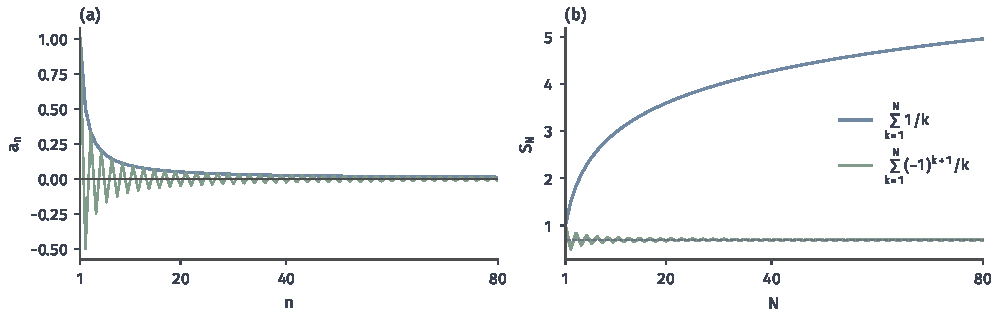
\includegraphics[width=169.0mm]{figures/01-mathematical-preliminaries-upper/01-mathematical-language-combinatorics-analysis-optimization/matplotlib/chapter3-concept-processes/series-terms-sums.pdf}
 \caption{(a) 蓝、绿折线分别连接$1/n$与$(-1)^{n+1}/n$的前80项。(b) 对应的部分和：调和部分和继续增长，交错调和部分和趋于虚线所示的$\log2$。项趋零只是级数收敛的必要条件；图展示有限段，收敛或发散由前面的判别证明。}
 \label{fig:analysis-process-series-terms-sums}
\end{figure*}

\subsubsection{级数的重排和分组对收敛的影响}

收敛判别确定了原次序下部分和的趋向。接下来改变求和的组织方式：重排改变各项的次序，
分组只把原次序中的有限个相邻项合并；两种操作对收敛性的影响不同，需要分别检验。

\paragraph{级数的重排}
有限和可以交换项的先后；无穷级数则要检查新的部分和如何覆盖旧项。
若$\pi:\{1,2,\ldots\}\to\{1,2,\ldots\}$为双射，$\sum_{n=1}^{\infty}a_{\pi(n)}$称为原级数的重排，
它每项恰好使用一次，改变的是各项进入累计的顺序。
对于非负项，任意有限选项的和都不超过原扩展总和；反过来，原来的任意前$N$项
也会全部进入重排的某个有限前段。对两个方向分别取上确界，便知重排保持总和，允许总和为$+\infty$。

绝对收敛也保证任意重排保持原和。
给定$\varepsilon>0$，先选$N$使$\sum_{n>N}|a_n|<\varepsilon$。
重排充分多项后已包含原来的前$N$项，而它选入或遗漏的其余贡献均来自这个绝对尾部。
将重排的有限和与原部分和比较，并让原部分和趋于$s$，误差至多为该绝对尾和，故重排仍趋于$s$。

条件收敛没有这一保证。设正项总和为$P$、负项绝对值总和为$Q$；
若其中一个有限，由$s_N=P_N-Q_N$收敛会推出另一个也有限，与绝对值和发散矛盾，
故二者都为$+\infty$。对任意实数目标$L$，可以依原先相对次序取正项直到部分和超过$L$，
再取负项直到低于$L$，反复进行；每次都至少取一项相应符号的项。
两类项最终都被用到，而$a_n\to0$使每次越过$L$的幅度趋零，因此可得到和为$L$的重排。
原级数若含零项，每轮再按原次序插入下一个尚未使用的零项（若有）；这不改变和，并保证每个零项也最终被用到。
也可交替超过$1$、低于$0$，构造不收敛的重排。
原来的和依赖抵消的顺序，不能只按有限和交换律任意调换。

\paragraph{级数的分组}
重排改变项的先后次序。若保留原次序，只将相邻的有限项合起来，则需要考察另一种改变求和方式的操作。
分组保持原项的顺序，只将有限个相邻项合为一项。
准确地说，取$0=n_0<n_1<n_2<\cdots$，令
$b_j=\sum_{k=n_{j-1}+1}^{n_j}a_k$，则分组后前$J$项的和恰为$s_{n_J}$。
所以原级数收敛到$s$时，分组后的部分和是原部分和的子序列，也必收敛到$s$；
这对绝对收敛和条件收敛都成立。

反向不成立。级数$1-1+1-1+\cdots$的部分和在$1$与$0$之间交替，原级数不收敛，
但按$(1-1)+(1-1)+\cdots$分组后各项为零。
分组只保留部分截断位置，可能掩盖块内的振荡。
非负项没有这种抵消：原部分和单调，分组截断又越过每一个原截断位置，
两者的上确界相同，故即使总和为$+\infty$也可保序分组。
结合非负重排规则，可先把非负项按任意编号排列，再分成有限相邻块，而不改变扩展总和；
后面的外测度构造将用这些求和性质累计覆盖区间的长度。

\FloatBarrier
\section{函数的极限}
\label{sec:analysis-function-limits}

数列的指标按自然数逐项增加，函数的输入却可以从许多实数位置靠近同一点。例如$(x^2-1)/(x-1)$在$x=1$没有定义，但在$x\neq1$时它等于$x+1$，所以邻近输入的输出仍趋于$2$。函数极限研究的正是这种去掉中心点后的共同趋近，不先要求函数在中心有取值。

\subsection{函数极限与单侧极限}
\paragraph{聚点}

讨论输入接近$a$之前，须保证定义域中确实有不同于$a$的输入能够任意靠近$a$。
设$X\subseteq\mathbb R$。若$a$的任意去心邻域都含有$X$中的点，
即每个$r>0$都能找到$x\in X$使$0<|x-a|<r$，就称$a$为$X$的聚点（cluster point）。
例如$0$是$(0,1)$的聚点，虽然$0$不属于这个集合；孤立点则不是聚点。
这个条件保证定义域中的点确实可以不断靠近$a$。

\paragraph{函数极限}
有了能够趋近的输入，还要用输入误差控制输出误差，这与数列极限比较尾部误差的思路相同。
设$f:X\to\mathbb R$，$a$为$X$的聚点。
若对每个$\varepsilon>0$，都存在$\delta>0$使
\[
 x\in X,\quad0<|x-a|<\delta\quad\Longrightarrow\quad|f(x)-b|<\varepsilon,
\]
就称$b$为$x\to a$时$f(x)$的极限，记作$\lim_{x\to a}f(x)=b$。
输入与$a$的距离足够小，便能保证输出与$b$的距离任意小。
定义中的$0<|x-a|$排除了中心点，所以既不要求$f(a)$有定义，也不要求它等于$b$。
例如$f(x)=(x^2-1)/(x-1)$在$x=1$没有定义，但对$x\neq1$有$f(x)=x+1$。
给定$\varepsilon>0$，取$\delta=\varepsilon$，则
$0<|x-1|<\delta$时$|f(x)-2|=|x-1|<\varepsilon$，所以其极限为$2$。


图~\ref{fig:analysis-process-epsilon-delta-band}将输入邻域与输出误差带对应起来，同时把基点取值与趋近时的极限分开。
\begin{figure}[!htbp]
 \centering
 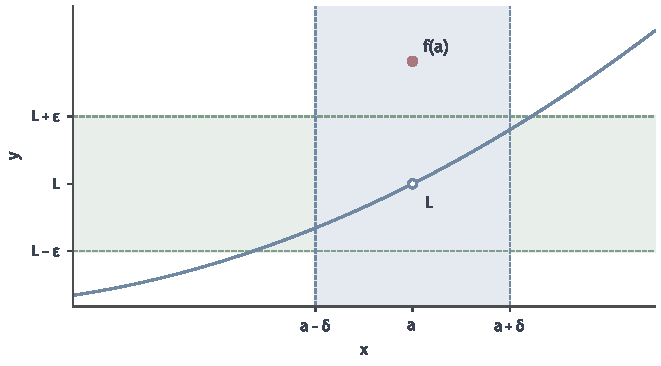
\includegraphics[width=112.0mm]{figures/01-mathematical-preliminaries-upper/01-mathematical-language-combinatorics-analysis-optimization/matplotlib/chapter3-concept-processes/epsilon-delta-band.pdf}
 \caption{取$a=L=1$，$x\neq1$时$f(x)=x^2$，另令$f(1)=2$。蓝带对应$\delta=0.2$的输入范围，绿带对应$\varepsilon=0.55$的输出范围；去掉$a$后，蓝带内曲线全部落在绿带内。空心点是极限位置，红实心点是$f(a)$，不参加去心邻域条件。}
 \label{fig:analysis-process-epsilon-delta-band}
\end{figure}

\paragraph{左极限与右极限}
实轴上的输入可以从一个点的两侧接近，而两侧的输出未必有相同趋向，因此先分别考察每一侧的极限。
只让$x<a$的点趋近$a$，得到左极限$\lim_{x\uparrow a}f(x)$；
只让$x>a$的点趋近$a$，得到右极限$\lim_{x\downarrow a}f(x)$。
两种定义分别在上述误差条件中增加$x<a$或$x>a$，
并要求相应一侧存在定义域中的点任意靠近$a$。
若两侧都能趋近$a$，双侧极限存在当且仅当左右极限都存在且相等。
例如$f(x)=\mathbb I\{x\geq0\}$在$0$处的左右极限分别为$0$和$1$，所以双侧极限不存在。
这里$\mathbb I$为指示函数：括号内条件成立时取$1$，否则取$0$。
在定义域$[a,b]$内，只能从右侧趋近左端点$a$，从左侧趋近右端点$b$。
这种左右判据依赖实轴上的顺序，多元函数还须控制其他趋近方式。

\paragraph{无穷远处的极限}
输入也可以趋于无穷。设定义域向右无界，条件
\[
 \lim_{x\to+\infty}f(x)=b
\]
表示：对每个$\varepsilon>0$，存在$M$，使定义域中所有$x>M$都满足$|f(x)-b|<\varepsilon$。
定义域向左无界时，$x\to-\infty$的定义相应要求所有$x<M$的允许输入满足同一误差界。
例如$1/x$在$x\to+\infty$和$x\to-\infty$时都趋于$0$。

\paragraph{值为无穷的极限}
前一段改变的是输入的趋向；即使输入趋近有限点，输出也可能越过任何有限界，因此还需要描述输出本身的无界趋向。
对有限聚点$a$，$f(x)\to+\infty$（$x\to a$）是指：对每个实数$M$，都存在$\delta>0$，使定义域中满足$0<|x-a|<\delta$的每个$x$都有$f(x)>M$。
趋于$-\infty$则把最后的不等式改为$f(x)<M$。单侧无穷极限再限制输入所在的一侧。因此$1/x$在$x\downarrow0$时趋于$+\infty$，在$x\uparrow0$时趋于$-\infty$，并没有共同的双侧无穷极限。

\subsection{常用极限}

\paragraph{三角函数的基本极限}
三角函数的自变量采用弧度制：单位圆上弧长为$h$的圆心角记为$h$。
比较内接三角形、扇形和外切三角形的面积，可得$0<h<\pi/2$时
$\sin h\leq h\leq\tan h$，从而$\cos h\leq\sin h/h\leq1$。
又由$1-\cos h=2\sin^2(h/2)\leq h^2/2$得到误差界
\[
 0\leq1-\frac{\sin h}{h}\leq1-\cos h\leq\frac{h^2}{2}.
\]
任给$\varepsilon>0$，只要$0<h<\min\{\pi/2,\sqrt{2\varepsilon}\}$，第一个比值与$1$的误差就小于$\varepsilon$。
同样由$|1-\cos h|/|h|\leq|h|/2$可控制第二个比值。因此
\[
 \lim_{h\to0}\frac{\sin h}{h}=1,
 \qquad
 \lim_{h\to0}\frac{\cos h-1}{h}=0.
\]
第一个比值是偶函数，所以右侧的论证也控制$h<0$；第二个误差界对正负两侧都适用。
弧度制使第一个极限恰为$1$，用角度制时会多出比例系数。

\paragraph{自然指数函数}
后面求指数函数的导数需要一个原点处的基本极限，因此先用级数构造自然指数函数，验证其收敛，再建立乘法性质和局部变化关系。
自然指数函数可由绝对收敛的级数构造：
\[
 \exp x=\sum_{k=0}^{\infty}\frac{x^k}{k!}.
\]
对固定$x$，充分靠后的相邻项绝对值之比不超过$1/2$，尾部被几何级数控制，所以级数收敛。
设两个级数的项分别为$a_k$与$b_j$。有限矩形和满足
$\sum_{k=0}^N\sum_{j=0}^Ma_kb_j=(\sum_{k=0}^Na_k)(\sum_{j=0}^Mb_j)$，
所以它们趋于两级数和的乘积。若两个级数都绝对收敛，双重和中各项的绝对值总和
由$(\sum_k|a_k|)(\sum_j|b_j|)$控制；舍去足够大的有限矩形后，剩余绝对尾和可任意小。
因此按总次数$k+j$合并，也得到同一极限。把这个结论用于指数级数，记
$C_n=\sum_{k=0}^n x^ky^{n-k}/[k!(n-k)!]$。将系数$n$拆为$k+(n-k)$，并分别换一次有限求和的索引，得到
\[
 nC_n=(x+y)C_{n-1},\qquad n\geq1.
\]
由$C_0=1$逐步得到$C_n=(x+y)^n/n!$，因而
\[
 \exp x\,\exp y
 =\sum_{n=0}^{\infty}\sum_{k=0}^n\frac{x^ky^{n-k}}{k!(n-k)!}
 =\sum_{n=0}^{\infty}\frac{(x+y)^n}{n!}
 =\exp(x+y).
\]
记$e=\exp1$，则$\exp x$就是以$e$为底的指数函数，通常写作$e^x$；$e$约为$2.71828$。
当$0<|h|<1/2$时，直接估计级数的二阶以后各项：
\[
 |e^h-1-h|
 \leq\sum_{k=2}^{\infty}|h|^k
 =\frac{h^2}{1-|h|}\leq2h^2.
\]
除以$|h|$并取极限，就有
\[
 \lim_{h\to0}\frac{e^h-1}{h}=1.
\]
这一推导先用级数构造指数函数，未使用求导或积分。
加法公式给出$e^xe^{-x}=1$以及$e^x=(e^{x/2})^2$，因此$e^x>0$。
对$u\geq0$，级数各项非负，只保留前两项便得
\[
 e^u\geq1+u\qquad(u\geq0),
\]
这正是第~\ref{chap:combinatorics}章简化Sauer--Shelah界时所用的不等式。
对$h>0$，由此$e^h\geq1+h>1$，于是$e^{x+h}=e^xe^h>e^x$，指数函数严格递增。
同一估计说明$x\to+\infty$时$e^x\to+\infty$；取倒数又得$x\to-\infty$时$e^x\to0$。
对固定$x$，上述余项界还给出$|e^{x+h}-e^x|\leq e^x(|h|+2h^2)\to0$。
这些性质将在连续函数的介值定理建立后，用于构造自然对数这一反函数
\scite{math-lebl-analysis1}。

\subsection{极限的性质与运算}
\paragraph{序列判据}

函数极限要求控制$a$附近所有允许的输入。这个条件等价于：每列满足$x_n\in X\setminus\{a\}$且$x_n\to a$的输入，都有$f(x_n)\to b$。正向把函数极限的同一个$\delta$用于序列尾部即可。反向若误差条件不成立，就存在$\varepsilon_0>0$，使每个$1/n$邻域内都能选到$x_n\neq a$，满足$|f(x_n)-b|\geq\varepsilon_0$；这列输入趋于$a$，输出却不趋于$b$，与序列条件矛盾。

\paragraph{和的极限}
序列判据把函数极限转化为数列极限，从而可以逐项建立函数极限的运算法则。
以下各段统一设$f,g:D\to\mathbb R$，$a$为$D$的聚点，且在$x\in D$、$x\to a$时
$f(x)\to b$、$g(x)\to c$，其中$b,c\in\mathbb R$。和的极限为
\[
 \lim_{x\to a}(f(x)+g(x))=b+c.
\]
任取$x_n\in D\setminus\{a\}$且$x_n\to a$，序列判据给出$f(x_n)\to b$、$g(x_n)\to c$；
数列和的法则给出$f(x_n)+g(x_n)\to b+c$。由于对任意这样的输入列都成立，再用序列判据即得结论。

\paragraph{差的极限}
相减也保留有限极限关系：
\[
 \lim_{x\to a}(f(x)-g(x))=b-c.
\]
对每列趋于$a$的允许输入，数列差的法则都给出相应输出差趋于$b-c$，再由序列判据返回函数极限。

\paragraph{数乘的极限}
固定倍数只按比例改变输出误差。对任意固定$\lambda\in\mathbb R$，
\[
 \lim_{x\to a}\lambda f(x)=\lambda b.
\]
沿任意允许输入列使用数列常数倍的极限，再用序列判据即可；$\lambda=0$时输出恒为零。

\paragraph{积的极限}
两个有限极限也可以分别相乘：
\[
 \lim_{x\to a}f(x)g(x)=bc.
\]
沿任意允许输入列应用数列乘积的法则，得到输出积趋于$bc$；序列判据保证这控制了$a$附近的全部允许输入。

\paragraph{商的极限}
商需要额外要求分母极限$c\neq0$，此时
\[
 \lim_{x\to a}\frac{f(x)}{g(x)}=\frac bc.
\]
先取输出误差$|c|/2$，便知$a$的某个去心邻域内有$|g(x)|>|c|/2>0$，商在那里有定义。
在这一邻域内，任意输入列都可使用数列的商法则，再由序列判据得到结论。
若分子分母都趋于零，就不能套用此式。例如$(x^2-1)/(x-1)$在$x\to1$时须先约去公因子$x-1$，才能求出极限$2$。
同样，$\infty-\infty$等形式也须先变形或另外估计。

\paragraph{夹逼定理}
不易直接分解的函数，可以用同趋向的两侧函数控制。设在$a$的某个去心邻域内，所有允许输入满足
$u(x)\leq h(x)\leq v(x)$，且$u(x)\to L$、$v(x)\to L$，其中$L\in\mathbb R$，则
\[
 \lim_{x\to a}h(x)=L.
\]
任给$\varepsilon>0$，取一个共同的输入邻域，使$u(x)$和$v(x)$都落在$(L-\varepsilon,L+\varepsilon)$内，
中间的$h(x)$也在其中。例如$-|x|\leq x\sin(1/x)\leq|x|$在$x\neq0$时成立，因此$x\to0$时$x\sin(1/x)\to0$。

\subsection{无穷小与无穷大}

\paragraph{无穷小}
趋向零的量可以出现在数列、函数或后面的微分余项中，先给这类趋向一个统一名称。
在指定的趋向下，极限为$0$的函数称为无穷小（infinitesimal）。
例如$x\to0$时，$x$和$x^2$都是无穷小；$n\to\infty$时，$1/n$也是无穷小。
“无穷小”描述变化过程中的极限性质，不是某个固定的很小的非零数。

\paragraph{无穷大}
函数值的绝对值也可能最终超过任意固定门槛，这种趋向与趋零可以通过倒数联系起来。
在指定的趋向下，若$|f(x)|\to+\infty$，则称$f$为无穷大。
例如$x\to0$时，$1/x$为无穷大，但它没有共同的正或负无穷极限。
若$f$在所考察范围内非零，则$|f|\to\infty$等价于$1/f\to0$。

\paragraph{渐近记号}
\label{sec:comb-growth-scales}
两个函数即使同为无穷小，趋零的相对速度也可以不同。
设在所讨论的趋向附近$g\neq0$，定义
\[
 f=o(g)\quad\text{表示}\quad \frac{f}{g}\longrightarrow0.
\]
这个小$o$记号表示$f$相对于$g$可以忽略。
若$|f/g|$在趋向附近有界，则记$f=O(g)$，称为大$O$记号。
大$O$只要求有常数$C$使$|f|\leq C|g|$最终成立，小$o$则要求这个相对比例趋于零。
例如$x\to0$时$x^2=o(x)$，而$3x=O(x)$但不是$o(x)$。
若$f/g\to1$，还记$f\sim g$，称为等价无穷小（当两者都趋零时）。
例如$x+x^2\sim x$，因为$(x+x^2)/x=1+x\to1$。

同样的记号可用于$n\to\infty$的数列：
$3n+7=O(n)$、$n/10=O(n)$，但这两个比值分别趋于$3$和$0.1$，所以都不是$o(n)$；
$10\sqrt n=o(n)$，因为$10\sqrt n/n=10/\sqrt n\to0$。
图~\ref{fig:vol1-add-asymptotic-ratios}画出这三个比值。

\begin{figure}[!htb]
  \centering
  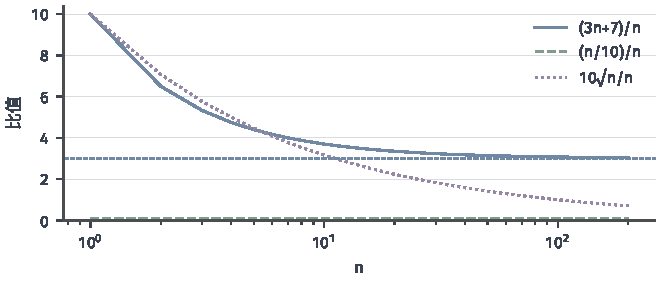
\includegraphics[width=112mm]{figures/01-mathematical-preliminaries-upper/01-mathematical-language-combinatorics-analysis-optimization/matplotlib/comprehension-additions/asymptotic-ratios.pdf}
  \caption{三个解析数列除以$n$后的比值，展示整数$n=1,\ldots,200$，横轴为对数刻度。蓝、绿、紫线的极限分别为$3,0.1,0$。前两者对应$O(n)$而非$o(n)$，第三者对应$o(n)$；极限由正文中的表达式判断，有限范围曲线只帮助观察。}
  \label{fig:vol1-add-asymptotic-ratios}
\end{figure}

对最终为正的数列，若存在$c>0$使$a_n\geq cb_n$最终成立，记$a_n=\Omega(b_n)$；
同时满足$a_n=O(b_n)$与$a_n=\Omega(b_n)$，记$a_n=\Theta(b_n)$，表示同一数量级。
例如$3n+7=\Theta(n)$。这里的常数不随趋于无穷的$n$改变。
$n=O(n^2)$也成立，因此大$O$给出上界，不一定给出精确的增长阶。
这些记号在求导和局部近似中用来表达余项的大小。

\FloatBarrier

\section{实数集与欧氏空间中的邻域和闭区间}
\label{sec:analysis-metric-measurement}
\label{sec:analysis-set-metric}

前两节的数列极限与函数极限都在控制距离：$|a_n-a|<\varepsilon$说明第$n$项离极限不远，
$0<|x-a|<\delta$说明输入离中心不远。本节先在实轴和有限维欧氏空间中把“一个点附近”写成开球与邻域，
再用邻域定义开集、闭集，并用点列刻画闭性；最后建立闭区间的有限子覆盖性质。
这些结论直接服务于下一章一元函数的连续性和极值，也服务于多元微积分中的欧氏集合。
把绝对值和欧氏范数抽象成任意集合上的度量，再讨论一般空间的完备性、可分性、全有界和紧致序列刻画，
是第~\ref{chap:metric-spaces}章“度量空间”的任务；本节不预设一般度量空间的结论。

\subsection{开球、邻域与开闭集}

\paragraph{开球与邻域}
讨论一个点附近的变化，需要先指定哪些对象算作离它足够近。给定中心和距离阈值后，可以把这些对象收集成一个集合。

\begin{definition}[欧氏开球]
\label{def:analysis-open-ball}
在$\mathbb R^d$中，以$\bm{x}$为中心、半径$r>0$的\term{开球}（open ball）记为
$B(\bm{x},r)=\{\bm{y}\in\mathbb R^d:\lVert\bm{y}-\bm{x}\rVert_2<r\}$。
当$d=1$时，$B(x,r)=(x-r,x+r)$就是开区间。
\end{definition}

开球把“离一个点足够近”写成集合。若集合$V$包含某个$B(\bm{x},r)$，就称$V$是$\bm{x}$的邻域；
邻域本身不必是开集。由这些邻域可以判断一个范围是否包含其中每个点附近的点。

图~\ref{fig:analysis-ball-neighborhood}将这两个对象分开：开球由距离直接确定，邻域则只需包含一个这样的开球。
\begin{figure}[htbp]
 \centering
 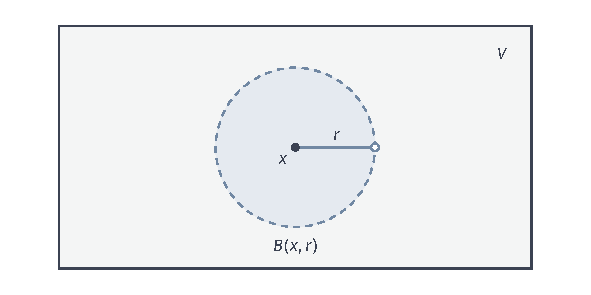
\includegraphics[width=\linewidth]{figures/01-mathematical-preliminaries-upper/01-mathematical-language-combinatorics-analysis-optimization/tikz/metric-ball-neighborhood/figure.pdf}
 \caption{平面欧氏距离下的开球与邻域。浅蓝圆盘为$B(\bm{x},r)$，虚线圆周不属于开球；灰色矩形$V$连同实线边界包含这个圆盘，因此是$\bm{x}$的邻域。$V$本身不是开集，说明“是某点的邻域”只要求在该点周围留有余量。}
 \label{fig:analysis-ball-neighborhood}
\end{figure}

\paragraph{开集与闭集}
有了开球，就能检验一个集合是否容纳其中每个点附近的一小片范围。对集合的补集作同样检验，又得到另一类常用的范围条件。

\begin{definition}[开集与闭集]
\label{def:analysis-open-closed-sets}
在$\mathbb R^d$中，集合$U$若对每个$\bm{x}\in U$都存在$r>0$使$B(\bm{x},r)\subseteq U$，就称为\term{开集}（open set）；
集合$F$若其补集$\mathbb R^d\setminus F$为开集，就称为\term{闭集}（closed set）。
\end{definition}

开闭性总是相对于当前空间而言。例如$[0,1/2)$在$\mathbb R$中不是开集，
但在子空间$X=[0,1]$中是开集：此时开球是实轴开区间与$X$的交，
$0$的一个小球不必包含负数。全集和空集既开又闭；“不是开集”也不等于“就是闭集”，实轴上的$[0,1)$便两者都不是。

图~\ref{fig:analysis-open-closed-relative}用端点附近的小球检验上述区别：实轴上包含端点的区间可能无法容纳小球，而在子空间中，小球本身也会随空间改变。
\begin{figure*}[htbp]
 \centering
 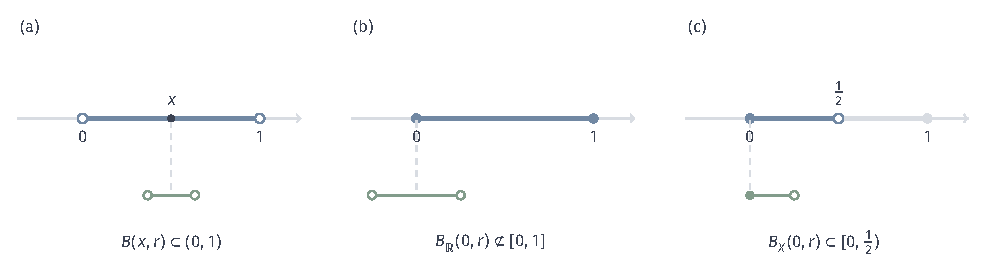
\includegraphics[width=169mm]{figures/01-mathematical-preliminaries-upper/01-mathematical-language-combinatorics-analysis-optimization/tikz/metric-open-closed-relative/figure.pdf}
 \caption{开集、闭集与所在空间。蓝色线段为待检验集合，绿色线段示意小球，空心端点排除、实心端点包含。(a) 在$\mathbb R$中，$(0,1)$的每个点都能选取一个包含于集合的小球，故为开集。(b) $[0,1]$在端点$0$处不能容纳任何实轴小球，因而不是开集；其补集$(-\infty,0)\cup(1,\infty)$为开集，故它是闭集。(c) 改在$X=[0,1]$中取球时，$B_X(0,r)=[0,r)$（$0<r<1/2$），因此$[0,1/2)$是$X$中的开集。图中只画出(c)的端点检验，其余点可直接沿用区间内部的小球。}
 \label{fig:analysis-open-closed-relative}
\end{figure*}

开球本身确实是开集：若$\bm{y}\in B(\bm{x},r)$，取$\rho=r-\lVert\bm{y}-\bm{x}\rVert_2>0$，
则三角不等式保证$B(\bm{y},\rho)\subseteq B(\bm{x},r)$。
任意多个开集的并仍开，因为并集中每个点都已属于某一个开集，可以沿用它的小球；
有限个开集的交仍开，因为可取各个允许半径的最小值。
无限多个开集的交则未必开，例如$\bigcap_{n\geq1}(-1/n,1/n)=\{0\}$。

\subsection{闭集的序列判据}

在欧氏空间中，闭集也可以用点列极限是否留在集合内来刻画。
$\mathbb R^d$中的点列$(\bm{x}_n)$收敛到$\bm{x}$，是指$\lVert\bm{x}_n-\bm{x}\rVert_2\to0$；
由于
\[
  |x_{n,j}-x_j|\leq\lVert\bm{x}_n-\bm{x}\rVert_2
  \leq\sqrt d\max_{1\leq j\leq d}|x_{n,j}-x_j|,
\]
欧氏距离收敛与有限个坐标同时收敛等价。

\begin{lemma}[闭集的序列判据]
\label{lem:analysis-closed-sequence-criterion}
设$F$为$\mathbb R^d$中的集合。$F$是闭集，当且仅当：对每个取值于$F$的点列$(\bm{x}_n)$，
若$\bm{x}_n\to\bm{x}$在$\mathbb R^d$中成立，则$\bm{x}\in F$。
\end{lemma}
\begin{proof}
若$F$闭而$\bm{x}\notin F$，开集$\mathbb R^d\setminus F$包含某个$B(\bm{x},r)$。
收敛要求充分靠后的$\bm{x}_n$落入这个球，与$\bm{x}_n\in F$矛盾。
反之，若$F$不闭，则存在$\bm{x}\in\mathbb R^d\setminus F$，使每个$B(\bm{x},r)$都与$F$相交。
为每个$n$选$\bm{x}_n\in F\cap B(\bm{x},1/n)$，便有$\bm{x}_n\to\bm{x}\notin F$，违反序列条件。
\end{proof}

例如$(0,1)$中的$1/n$在$\mathbb R$中趋于$0$，而$0\notin(0,1)$，所以$(0,1)$不是实轴中的闭集；
改在子空间$(0,1)$中判断时，$0$已不是环境中的候选极限。闭与有界描述的也是不同性质：
$(0,1)$有界但不闭，$\mathbb R$闭但不有界。

\subsection{闭区间的有限子覆盖性质}

\paragraph{开覆盖与有限子覆盖}

连续性在每一点给出一个邻域内的控制，但不同点的邻域大小可能不同。
要得到对整个闭区间同时有效的结论，需要从无限多个邻域中选出有限个，仍覆盖整个区间；
测量区间长度时也会遇到同样的问题：用可数多个开区间覆盖闭区间后，希望只保留其中有限个。
下面先规定“从一族开集中选出有限部分仍不遗漏”的含义。
\begin{definition}[开覆盖与紧致性]
\label{def:analysis-compactness}
设$K\subseteq\mathbb R^d$。一族开集的并包含$K$时，称它们为$K$的\term{开覆盖}（open cover）；
从中选出的有限个开集仍覆盖$K$时，称它们构成\term{有限子覆盖}（finite subcover）。
若$K$的每个开覆盖都存在有限子覆盖，则称$K$\term{紧致}（compact）。
\end{definition}
开覆盖本身可以有无限多个成员；有限子覆盖要求从原来的成员中挑选，而不是另换一组集合。

\paragraph{闭区间的紧致性}

闭区间里的点不会逃向无穷，收敛子列的极限也不会离开区间。
这两个条件使局部邻域覆盖不能一直要求加入新的成员。
\begin{theorem}[闭区间的有限子覆盖性质]
\label{thm:analysis-interval-finite-subcover}
实轴上的每个闭区间$[a,b]$都是紧致集。
\end{theorem}
\begin{proof}
$a=b$时选择一个包含该点的覆盖成员即可。设$a<b$，并给定$[a,b]$的开覆盖$\mathcal U$。
先证明这组覆盖有一个共同尺度：
\begin{equation}
 \exists r>0,\quad\forall x\in[a,b],\quad\exists U\in\mathcal U,
 \qquad B(x,r)\cap[a,b]\subseteq U.
\label{eq:analysis-cover-uniform-radius}
\end{equation}
若不存在这样的$r$，对每个$n$可选$x_n\in[a,b]$，使
$B(x_n,1/n)\cap[a,b]$不包含于任何一个覆盖成员。
有界数列$(x_n)$有子列$x_{n_k}\to x\in[a,b]$。
选$U\in\mathcal U$包含$x$，由开性取$\rho>0$使$B(x,\rho)\subseteq U$。
当$k$足够大时，$|x_{n_k}-x|<\rho/2$且$1/n_k<\rho/2$，
于是$B(x_{n_k},1/n_k)\subseteq B(x,\rho)\subseteq U$，产生矛盾。

有了共同半径$r$，把$[a,b]$分成有限个长度小于$r$的小区间。
每段任选一个点$x$，整段都落在$B(x,r)\cap[a,b]$内，故可由一个覆盖成员包含。
每段选择一个这样的成员，得到有限子覆盖。
\end{proof}

每个有界闭集$K\subseteq\mathbb R$也有此性质：先把它放入某个$[a,b]$，
再把$\mathbb R\setminus K$加入它的任意开覆盖，应用闭区间结论后删去这一补集。
在有限维欧氏空间$\mathbb R^d$中，闭且有界的集合同样紧致：逐次对各坐标使用Bolzano--Weierstrass定理，
可以从任意有界点列中选出在$\mathbb R^d$内收敛的子列，闭集的序列判据再把极限留在集合内；
这一序列刻画与开覆盖紧致性在一般度量空间中的等价证明，留到第~\ref{chap:metric-spaces}章。
有限子覆盖控制的是整个集合，而非只在几个已选点附近留出余量。图~\ref{fig:analysis-process-finite-open-cover}对照一个闭区间的有限覆盖与一个开区间上无法有限选取的覆盖族。
\begin{figure}[!htbp]
 \centering
 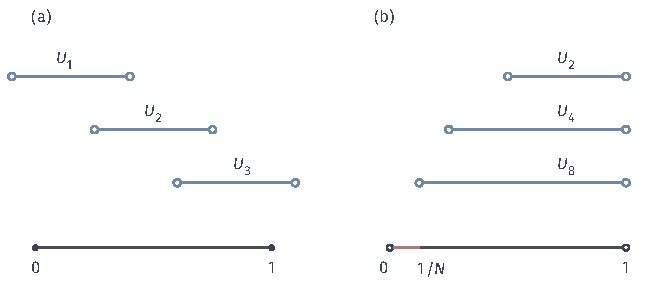
\includegraphics[width=112mm]{figures/01-mathematical-preliminaries-upper/01-mathematical-language-combinatorics-analysis-optimization/tikz/chapter3-concept-processes/finite-open-cover.pdf}
 \caption{(a) 三个开区间$(-0.1,0.4)$、$(0.25,0.75)$、$(0.6,1.1)$覆盖$[0,1]$。(b) $U_n=(1/n,1)$（$n\geq2$）覆盖$(0,1)$；只选有限多个时，设最大下标为$N$，红段$(0,1/N]$仍未覆盖。图只画$U_2,U_4,U_8$；右侧的失败由最大下标论证，不是有限图像的猜测。}
 \label{fig:analysis-process-finite-open-cover}
\end{figure}

\FloatBarrier


\FloatBarrier
\section{本章小结}
\label{sec:function-limits-summary}

$|\rho|<1$时等比序列趋于零，有限几何和趋于$1/(1-\rho)$。
极限先规定趋近的含义，再分别研究怎样计算极限、怎样保证极限存在；后者依赖实数的确界原理。
级数把累计过程写成部分和的极限；重排改变项的顺序，分组保留次序而合并相邻项，二者的结论不能混用。
度量规定点之间的距离，开集、闭集、完备性与紧致性由距离描述。
闭区间的紧致性使局部控制能够合成整体控制，后续微积分将据此研究连续性、变化与累计。

